% Author Name: José Areia 
% Author Contact: jose.apareia@gmail.com
% Version: 2.2.10 - 2025-07-18
% Public Repository: https://github.com/joseareia/ipleiria-thesis
% Wiki/Getting Help: https://github.com/joseareia/ipleiria-thesis/wiki

%%% Document Options %%%
\documentclass[
    language=french,
    school=eniad,
    docstage=final,
    media=paper,
    bookprint=false,
    linkcolor=red!45!black,
    chapterstyle=classic,
    coverstyle=classic,
    aiack=true
]{IPLeiriaThesis} % Refer to the Wiki for a list of available options.

%%% Document Version %%%
\DocumentVersion{1.0.0} % Required only if the 'docstage' is set to 'working'.

%%% Document Metadata %%%
% First Author (Mandatory)
\FirstAuthor{AbdElMalek Lamkadem}
% \FirstAuthorNumber{2230455}

% Second Author (Optional)
\SecondAuthor{Jane Smith}
% \SecondAuthorNumber{2230456}

% Third Author (Optional)
\ThirdAuthor{July Smith}
% \ThirdAuthorNumber{2230457}

% Supervisor (Mandatory)
\Supervisor{John Smith}
\SupervisorMail{joe.smith@ipleiria.pt}
% Please provide: [Current Title, Affiliation]
\SupervisorTitle{Full Professor, Polytechnic of Leiria} 

% Co-Supervisor (Optional)
% \CoSupervisor{Steve Smith}
% \CoSupervisorMail{steve.smith@ipleiria.pt}
% \CoSupervisorTitle{Associate Professor, Polytechnic of Leiria}

% Second Co-Supervisor (Optional)
% \SecCoSupervisor{Shak Smith}
% \SecCoSupervisorMail{shak.smith@ipleiria.pt}
% \SecCoSupervisorTitle{Associate Researcher, Computer Science \& Communication Research Centre}

% Title (Mandatory)
\Title{rapport de stage pfa a majal berkane}

% Subtitle (Mandatory)
\Subtitle{developpement de aquadrone une unmanned surface vehicle}

% University (Mandatory)
\University{universitie mohamed premier}

% School (Mandatory)
\School{ecole national de lintelegence artificiel et digital}

% Department (Mandatory)
% \Department{Department of Computer Engineering}

% Degree (Mandatory)
\Degree{robotique \&objects connectes}

% Course (Optional)
% \Course{Offensive \& Defensive Cybersecurity}

% Thesis Theme (Mandatory)
\ThesisType{stage }

% Local & Date (Mandatory)
\Date{Berkane, \DTMmonthname{\month} \number\year}

% Academic Year 
\AcademicYear{2024/25}

%%% Loading of Glossary and Acronyms %%%
\makeglossaries
\loadglsentries{Matter/05-Glossary}
\loadglsentries[\acronymtype]{Matter/06-Acronyms}
\loadglsentries[\symboltype]{Matter/07-Symbols}

\begin{document}

%%% Front Matter %%%
\ifthenelse{\equal{\getLanguage}{portuguese}}{%
    \pdfbookmark[0]{Capa}{capa} % Add entry to PDF bookmarks group.
    \pdfbookmark[1]{Frontispício}{frontispício} % Add entry to PDF.
}{%
    \pdfbookmark[0]{Front Matter}{frontmatter} % Add entry to PDF bookmarks group.
    \pdfbookmark[1]{Cover}{cover} % Add entry to PDF.
}

% Add background picture depending on the 'bwcover' variable.
\ifbwcover
    \newcommand\BackgroundPicCover{%
    \put(0,0){%
    \parbox[b][\paperheight]{\paperwidth}{%
    \vfill
    \centering
    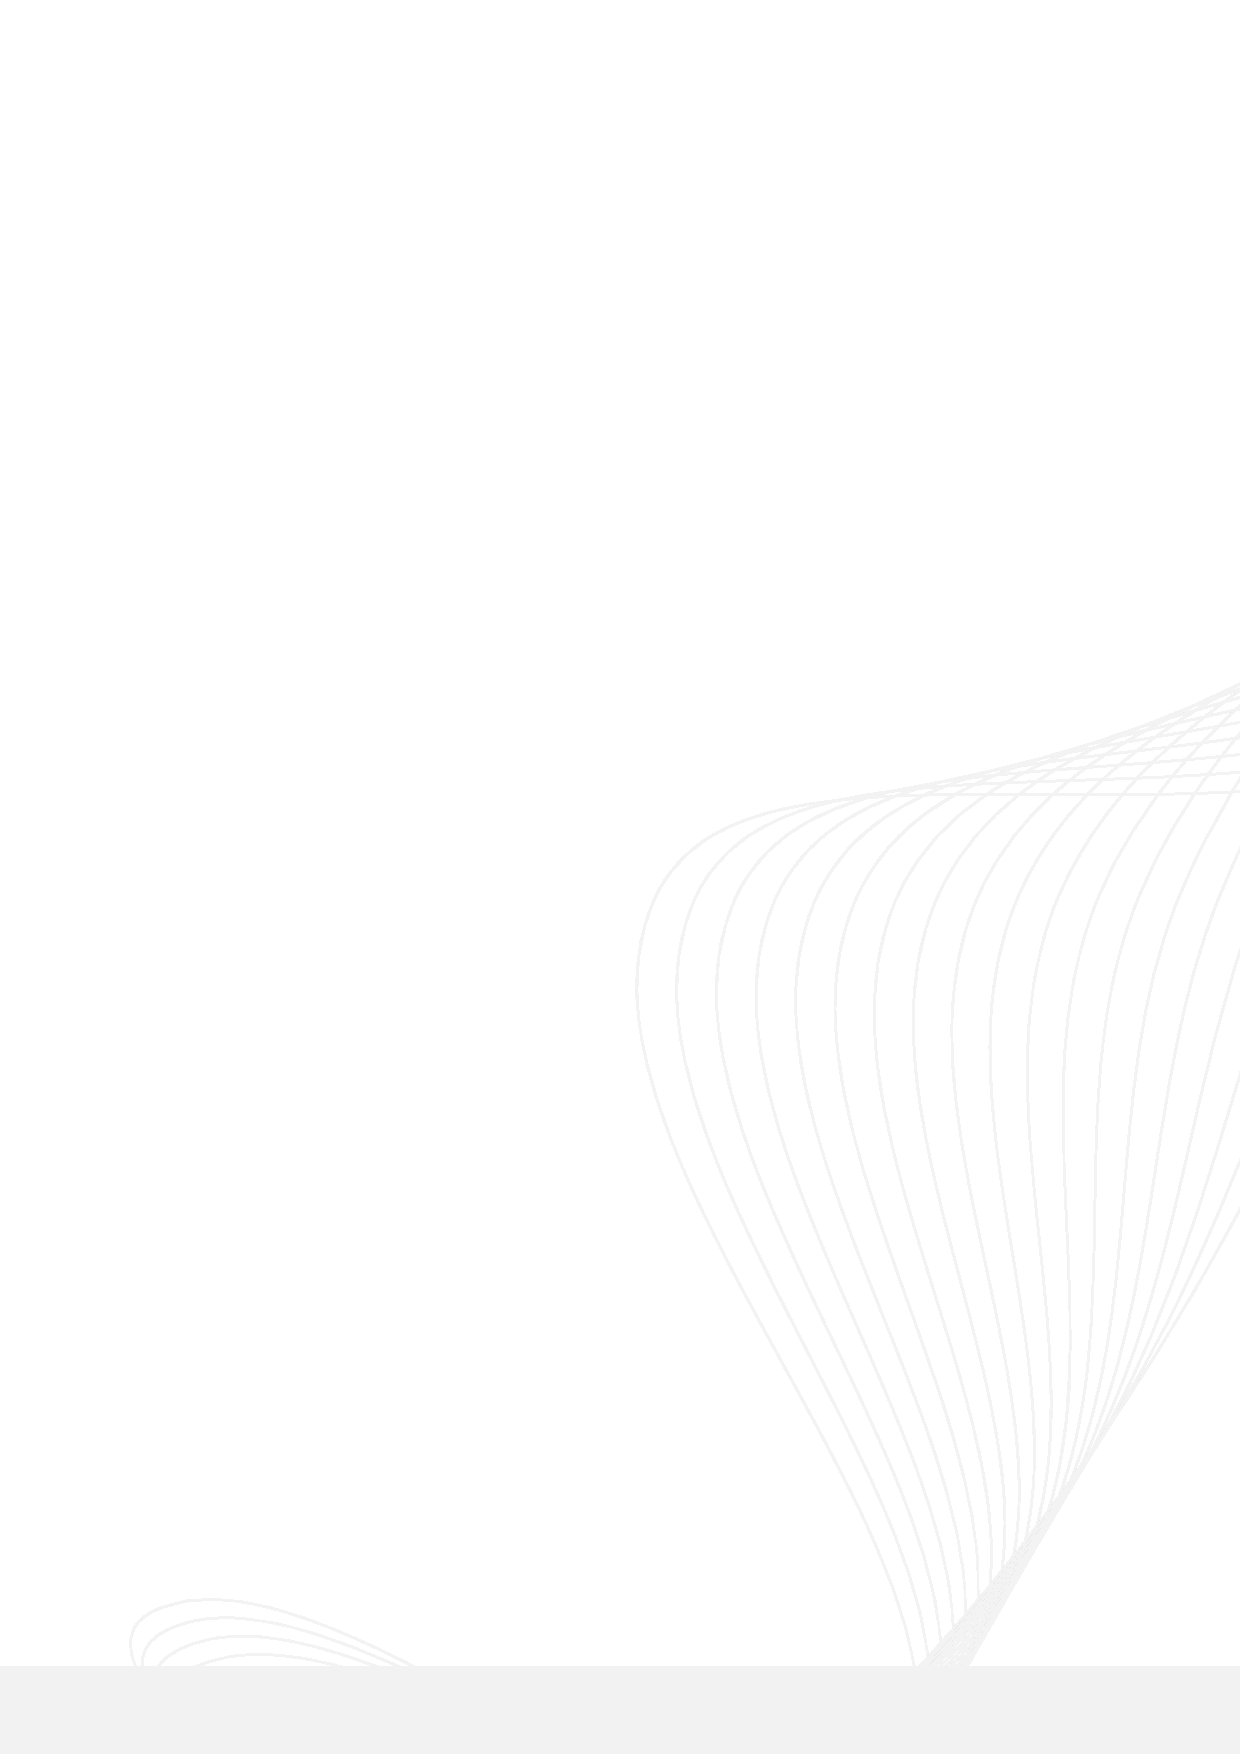
\includegraphics[width=\paperwidth,height=\paperheight,keepaspectratio]{Figures/Theme/Front-Page-BG.pdf}%
    \vfill
    }}}
\else
    \newcommand\BackgroundPicCover{%
    \put(0,0){%
    \parbox[b][\paperheight]{\paperwidth}{%
    \vfill
    \centering
    
\includegraphics[width=\paperwidth,height=\paperheight,keepaspectratio]{Figures/Theme/Cover-BG.pdf}%
    \vfill
    }}}
\fi

\AddToShipoutPictureBG*{\BackgroundPicCover}

\newgeometry{margin=1.98cm, top=2.15cm, bottom=1.47cm}
\begin{titlepage}
    \latofont % Switch to Lato font for the title page.
   
    \ifbwcover
        \color{frontpagedark} % Define the color to use within this page.
    \else
        \color{white} % Define the color to use within this page.
    \fi
    
    \vspace*{\baselineskip} % White space at the top of the page.

    \ifbwcover
        \begin{figure}
            
\includegraphics[width=0.32\linewidth]{Figures/Theme/IPLeiria-Logo-B.pdf}
        \end{figure}
    \else
        \begin{figure}
            
\includegraphics[width=0.32\linewidth]{Figures/Theme/IPLeiria-Logo-W.pdf}
        \end{figure}
    \fi

    \vspace{5.5\baselineskip}

    % Title
	\noindent
    \makebox[\textwidth][l]{%
        \parbox{\dimexpr\textwidth-2.5cm\relax}{
            \setstretch{1.03}
            \raggedright\bfseries\fontsize{20}{26}\selectfont\thetitle
        }
    }

    \vspace{0.8\baselineskip}

    % Subtitle
    \noindent
    \makebox[\textwidth][l]{%
        \parbox{\dimexpr\textwidth-7cm\relax}{
            \setstretch{1.03}
            \raggedright\fontsize{14}{19}\selectfont\subname
        }
    }

    \vspace{35pt}  

    % Author
    {\noindent\bfseries\fontsize{14}{19}\selectfont\firstauthorname}

    \ifdefined\secondauthorname
        \vspace{8pt}
        {\noindent\bfseries\fontsize{14}{19}\selectfont\secondauthorname}
	\fi

    \ifdefined\thirdauthorname
        \vspace{8pt}
        {\noindent\bfseries\fontsize{14}{19}\selectfont\thirdauthorname}
	\fi
 
	\vfill

    % School
	{\noindent\fontsize{10}{12}\selectfont\schoolname}
	
    % Department
	{\noindent\fontsize{10}{12}\selectfont\departmentname}

    % Degree
	{\noindent\fontsize{10}{12}\selectfont\degname}

    % Course
    \ifdefined\coursename
        {\noindent\fontsize{10}{12}\selectfont\coursename}
	\fi

    \vspace{125pt}

    % Local & Date
	{\noindent\fontsize{10}{12}\selectfont\thedate}

    \vspace{68pt}
\end{titlepage}
\restoregeometry\blankpage
\newcommand\BackgroundPicFrontPage{%
    \put(0,0){%
    \parbox[b][\paperheight]{\paperwidth}{%
    \vfill
    \centering
    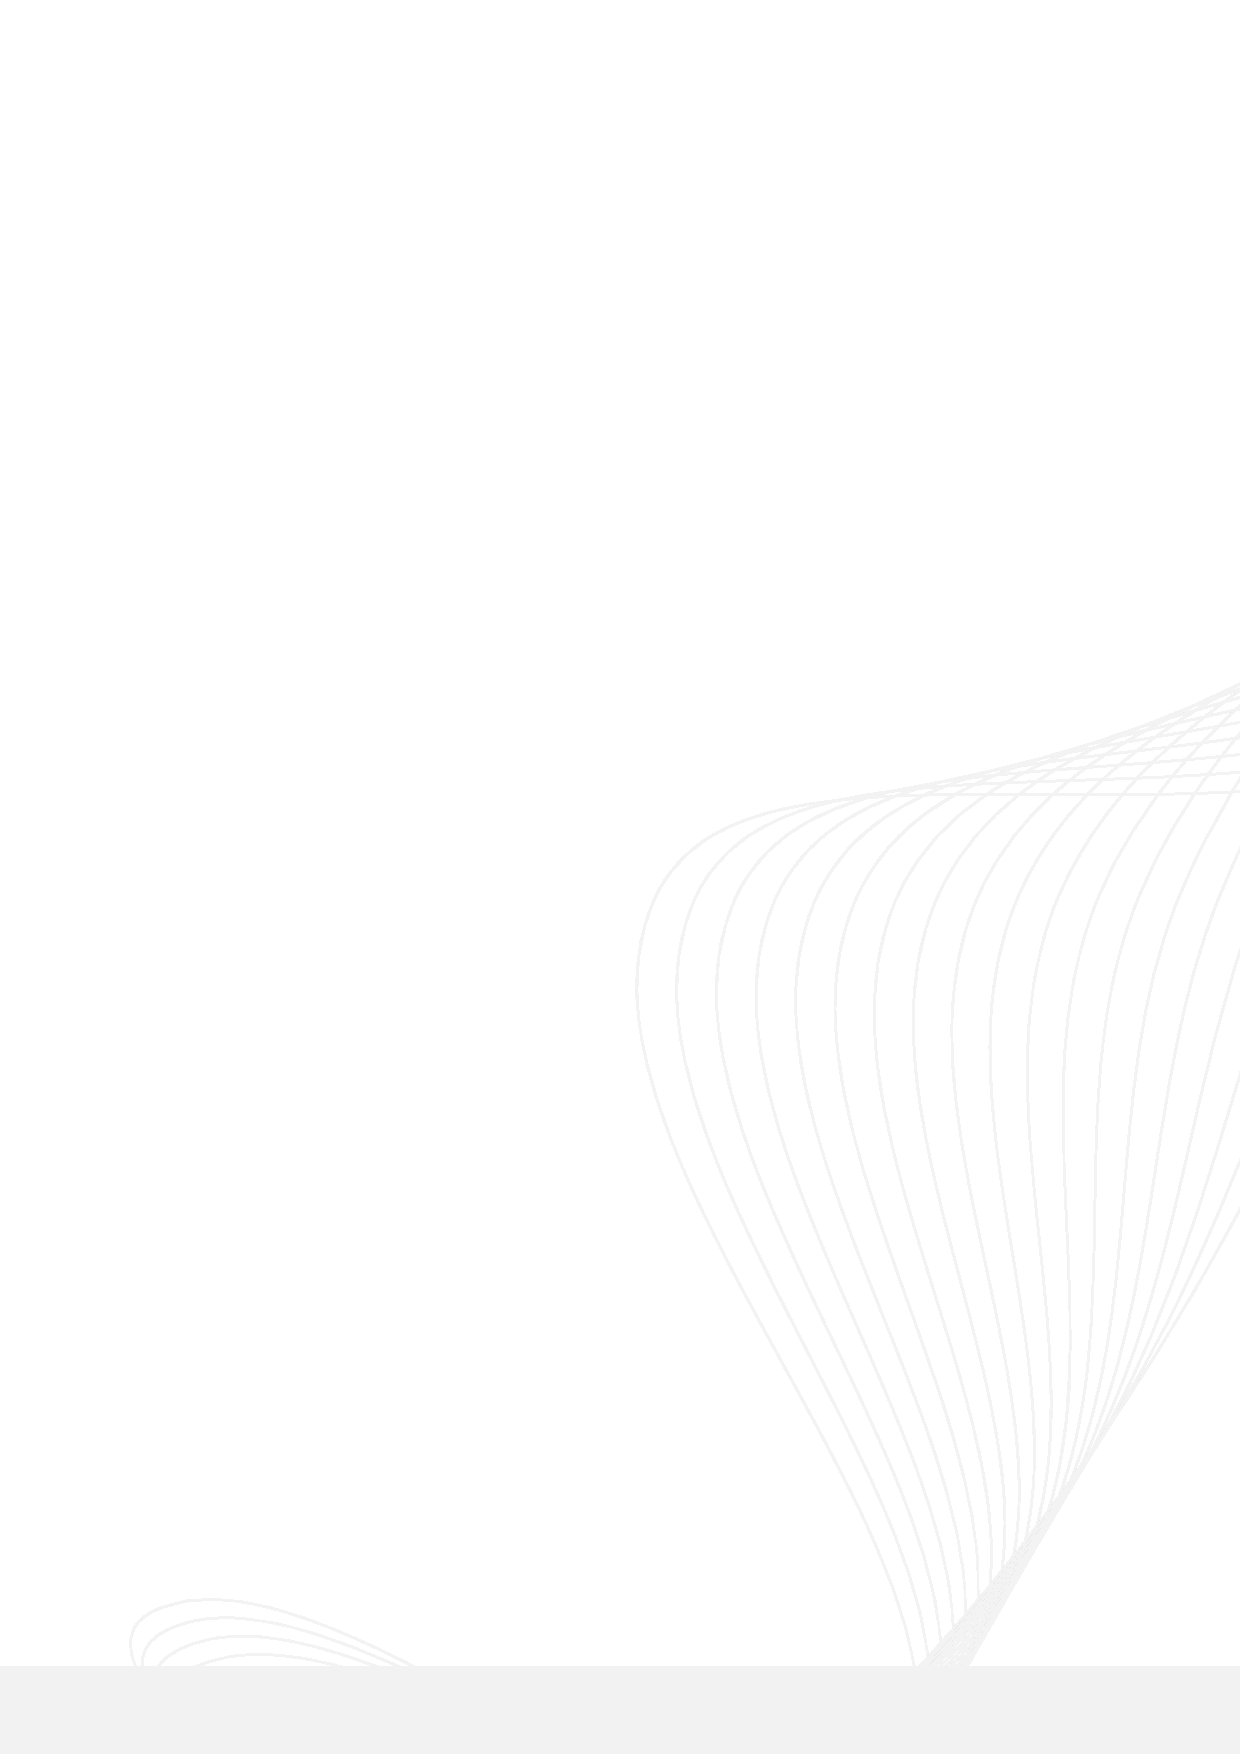
\includegraphics[width=\paperwidth,height=\paperheight,keepaspectratio]{Figures/Theme/Front-Page-BG.pdf}%
    \vfill
}}}
\AddToShipoutPictureBG*{\BackgroundPicFrontPage}

\newgeometry{margin=1.98cm, top=2.15cm, bottom=1.47cm}
\begin{titlepage}
    \latofont
    \color{frontpagedark}
    \vspace*{\baselineskip}

    \ifthenelse{\equal{\SchoolOption}{estg}}{
        \begin{figure}
            
\includegraphics[width=0.485\linewidth]{Figures/Theme/Logotypes/IPLeiria-ESTG-Logo-B.pdf}
        \end{figure}
    }
    
    \ifthenelse{\equal{\SchoolOption}{esad}}{
        \begin{figure}
            
\includegraphics[width=0.485\linewidth]{Figures/Theme/Logotypes/IPLeiria-ESAD-Logo-B.pdf}
        \end{figure}
    }
    
    \ifthenelse{\equal{\SchoolOption}{esslei}}{
        \begin{figure}
            
\includegraphics[width=0.485\linewidth]{Figures/Theme/Logotypes/IPLeiria-ESSLEI-Logo-B.pdf}
        \end{figure}
    }
    
    \ifthenelse{\equal{\SchoolOption}{estm}}{
        \begin{figure}
            
\includegraphics[width=0.485\linewidth]{Figures/Theme/Logotypes/IPLeiria-ESTM-Logo-B.pdf}
        \end{figure}
    }
    
    \ifthenelse{\equal{\SchoolOption}{esecs}}{
        \begin{figure}
            
\includegraphics[width=0.485\linewidth]{Figures/Theme/Logotypes/IPLeiria-ESECS-Logo-B.pdf}
        \end{figure}
    }

    \vspace{3.5\baselineskip}

    % Title.
	\noindent
    \makebox[\textwidth][l]{%
        \parbox{\dimexpr\textwidth-2.5cm\relax}{
            \setstretch{1.03}
            \raggedright\bfseries\fontsize{20}{26}\selectfont\GetTitle
        }
    }

    \vspace{0.8\baselineskip}

    % Subtitle.
    \noindent
    \makebox[\textwidth][l]{%
        \parbox{\dimexpr\textwidth-7cm\relax}{
            \setstretch{1.03}
            \raggedright\fontsize{14}{19}\selectfont\GetSubtitle
        }
    }

    \vspace{35pt}

    % Author.
    {\noindent\bfseries\fontsize{14}{19}\selectfont\GetFirstAuthor}
    
    {\noindent\itshape\fontsize{10}{10}\selectfont Student No. \GetFirstAuthorNumber}

    \ifdefined\GetSecondAuthor
        \vspace{8pt}
        {\noindent\bfseries\fontsize{14}{19}\selectfont\GetSecondAuthor}
	\fi

    \ifdefined\GetThirdAuthor
        \vspace{8pt}
        {\noindent\bfseries\fontsize{14}{19}\selectfont\GetThirdAuthor}
	\fi

    \vspace{58pt}    

    {
    \noindent
    \latofont
    \fontsize{10}{12}\selectfont
    \renewcommand{\arraystretch}{0.1}
    \hspace*{-2.5pt}\begin{tabular}{@{}r@{\hspace{5pt}}>{\raggedright\arraybackslash}m{6cm}@{}}
        \textbf{Supervisor:} & \GetSupervisor \\ [-.7ex]
        & \setstretch{0.9}{\fontsize{8}{10}\selectfont\itshape \GetSupervisorTitle} \\ [2ex]
        
        \ifdefined\GetCoSupervisor
            \textbf{Co-supervisor:} & \GetCoSupervisor \\ [-.7ex]
            & \setstretch{0.9}{\fontsize{8}{10}\selectfont\itshape \GetCoSupervisorTitle} \\ [.5ex]
        \fi

        \ifdefined\GetSecCoSupervisor        
            & \GetSecCoSupervisor \\ [-.7ex]
            & \setstretch{0.9}{\fontsize{8}{10}\selectfont\itshape \GetSecCoSupervisorTitle} \\
        \fi
    \end{tabular}
    }
    
    \vfill
	
    % School.
	{\noindent\fontsize{10}{12}\selectfont\GetSchool}
	
    % Department.
	{\noindent\fontsize{10}{12}\selectfont\GetDepartment}

    % Degree.
	{\noindent\fontsize{10}{12}\selectfont\GetDegree}

    % Course.
    \ifdefined\GetCourse
        {\noindent\fontsize{10}{12}\selectfont\GetCourse}
	\fi

    \vspace{45pt}

    % Thesis option.
	{\noindent\fontsize{10}{12}\itshape\selectfont\GetThesisType}

    \vspace{45pt}

    % Local and date.
	{\noindent\fontsize{10}{12}\selectfont\GetDate}

    \vspace{68pt}
\end{titlepage}
\restoregeometry
\MediaOptionLogicBlank

%%% Roman Numeration %%%
\pagenumbering{roman}

%%% Acknowledgements %%%
\ifthenelse{\equal{\LanguageOption}{portuguese}}{%
    \chapter*{Agradecimentos}
}{%
    \chapter*{Acknowledgements}
}

In the \textit{Acknowledgment} section, express your gratitude to those who helped and supported your work. Start by thanking your advisors, mentors, or supervisors who provided guidance and expertise. Mention any colleagues, classmates, or team members who contributed to discussions or offered assistance. You can also acknowledge specific organisations, institutions, or funding sources that supported your research or work. Lastly, include any personal acknowledgments for family or friends who offered encouragement and moral support during the project. Keep this section sincere, concise, and professional.

\plainblankpage

%%% Abstract %%%
\thispagestyle{plain}


% English Abstract 
\pdfbookmark[1]{Abstract}{abstract}
\chapter*{Abstract}
\guideinfo{In the \textit{Abstract} section, provide a concise summary of your project, highlighting the key points. Begin with a brief statement of the problem or objective, followed by a description of your approach or methodology. Summarise the main results or findings, emphasising their significance or implications. Conclude with a sentence or two on the overall contribution or impact of your work. Keep the abstract clear and focused, ideally within 150-250 words, to give readers a quick understanding of your research and its importance.}
\keywordsen{Keyword A, Keyword B, Keyword C.}
\MediaOptionLogicBlank

% French Abstract 
\pdfbookmark[1]{Résumé}{resume}
\chapter*{Résumé}
\guideinfo{Dans la section \textit{Résumé}, présentez un résumé concis de votre projet en mettant en avant les points clés. Commencez par une brève déclaration du problème ou de l'objectif, suivie d'une description de votre approche ou méthodologie. Résumez les principaux résultats ou conclusions en soulignant leur importance ou leurs implications. Concluez par une ou deux phrases sur la contribution globale ou l'impact de votre travail. Le résumé doit être clair et concis (idéalement 150-250 mots) pour permettre aux lecteurs de comprendre rapidement votre travail et son importance.}
\keywordsen{Mot-clé A, Mot-clé B, Mot-clé C.}
\MediaOptionLogicBlank

% Arabic Abstract 
% \pdfbookmark[1]{ملخص}{abstract-ar}
% \chapter*{ملخص}
% \guideinfo{في قسم \textit{الملخص}، قدّم ملخصًا موجزًا لمشروعك مع إبراز النقاط الرئيسية. ابدأ ببيان مختصر للمشكلة أو الهدف، يليه وصف لمنهجيتك أو طريقة بحثك. لخّص النتائج أو الاستنتاجات الرئيسية مع التأكيد على أهميتها أو تداعياتها. اختتم بجملة أو جملتين حول الإسهام العام أو تأثير عملك. يجب أن يكون الملخص واضحًا وموجزًا (150-250 كلمة مثاليًا) لتمكين القراء من فهم عملك وأهميته بسرعة.}
% \keywordspt{كلمة مفتاحية أ، كلمة مفتاحية ب، كلمة مفتاحية ج.}
% \MediaOptionLogicBlank

%%% AI Acknowledgement %%%
\ifthenelse{\equal{\AiAckOption}{true}}{%
    \ifthenelse{\equal{\LanguageOption}{portuguese}}{%
        \chapter*{Declaração sobre o Uso de Inteligência Artificial}

        \guideinfo{É uma boa prática académica indicar brevemente como, porquê e quando a IA foi utilizada. Explicar as ações tomadas e as razões que lhes estão subjacentes promove a reflexão crítica, aprofunda a compreensão do papel da IA na aprendizagem e ajuda a avaliar o seu impacto na qualidade e integridade do trabalho. Esta página pode ser removida definindo a opção \texttt{aiack} como \texttt{false} nas opções da classe do documento.}
    
        \vspace{2em}
        
        \exampleinfo{%
        Reconheço a utilização do ChatGPT (\url{https://chatgpt.com}) para aperfeiçoar o tom académico e melhorar a precisão linguística deste trabalho, incluindo aspectos de gramática, pontuação e vocabulário.
        
        \vspace{1em}
        
        \noindent\textbf{Descrição da Utilização}
        
        \prompt[1]{Num parágrafo, descreva simplesmente o que é o LaTeX.}
        
        \aioutput[1]{O LaTeX é um sistema de composição de alta qualidade, normalmente utilizado para produzir documentos científicos e matemáticos, devido ao seu poderoso manuseamento de fórmulas e bibliografias. Ao contrário dos processadores de texto, utiliza ficheiros de texto simples com etiquetas de marcação para definir a estrutura e a formatação de um documento, permitindo um controlo preciso da disposição e do aspeto. É especialmente popular no meio académico e na investigação para a criação de teses, artigos de revistas e apresentações.}
        }
    }{%
        \chapter*{AI Acknowledgement}

        \guideinfo{It is good academic practice to briefly state how, why, and when AI was used. Explaining both the actions taken and the reasons behind them encourages critical reflection, deepens understanding of AI's role in learning, and supports the evaluation of its impact on your work’s quality and integrity. This page can be removed by setting the option \texttt{aiack} to \texttt{false} in the document class options.}

        \vspace{2em}
        
        \exampleinfo{%
        I acknowledge the use of ChatGPT (\url{https://chatgpt.com}) to refine the academic tone and improve the linguistic accuracy of this work, including aspects of grammar, punctuation, and vocabulary.
        
        \vspace{1em}
        
        \noindent\textbf{Description of Use}
        
        \prompt[1]{In a paragraph, simply describe what LaTeX is.}
        
        \aioutput[1]{LaTeX is a high-quality typesetting system commonly used for producing scientific and mathematical documents due to its powerful handling of formulas and bibliographies. Unlike word processors, it uses plain text files with markup tags to define the structure and formatting of a document, allowing precise control over layout and appearance. It is especially popular in academia and research for creating theses, journal articles, and presentations.}
        }
    }
    
    \MediaOptionLogicBlank   
}{}

%%% Table of Contents, List of Figures and List of Tables %%%
\bookmarktocentry\tableofcontents
\listoffigures
\listoftables

%%% Print: Glossary and Acronyms %%%
\glossarytoc\printnormalglossary
\acronymtoc\printacronymglossary
\symboltoc\printsymbolglossary

%%% Arabic Numeration %%%
\pagenumbering{arabic}

%%% Main Chapters %%%
\chapter[Introduction générale]{Introduction générale}
\label{cp:introduction-generale}

{
\parindent0pt

\section{Contexte du projet et importance dans le domaine maritime}
Le domaine maritime représente un enjeu crucial pour l'économie mondiale, la sécurité et la préservation de l'environnement. La surveillance des océans, la gestion des ressources halieutiques et la protection des écosystèmes marins nécessitent des solutions innovantes et adaptées aux défis spécifiques de l'environnement marin.

Les technologies autonomes et la robotique maritime émergent comme des solutions prometteuses pour répondre à ces défis. Les véhicules de surface sans équipage (USV - Unmanned Surface Vehicles) offrent de nouvelles possibilités pour la surveillance maritime, la collecte de données océanographiques et l'assistance à la pêche, tout en réduisant les risques pour les équipages humains.

\begin{block}[note]
Cette introduction présente le cadre général du projet AquaDrone, un véhicule autonome multifonction développé pour répondre aux défis spécifiques de l'environnement maritime marocain et méditerranéen.
\end{block}

\section{Problématique générale}
Malgré les avancées technologiques récentes, les systèmes nautiques actuels présentent plusieurs limitations qui freinent leur adoption généralisée et leur efficacité opérationnelle. Les défis incluent la robustesse face aux conditions marines difficiles, l'autonomie énergétique limitée, la fiabilité des communications en mer et l'intégration harmonieuse de multiples capteurs et systèmes.

La complexité de l'environnement maritime - caractérisé par des conditions météorologiques variables, la corrosion saline, et les contraintes de navigation - nécessite des solutions techniques robustes et adaptées.

\section{Objectifs globaux}
Ce projet vise à développer un véhicule autonome multifonction capable de :
\begin{itemize}
    \setlength{\itemsep}{.375em}
    \item Assurer la surveillance maritime continue et autonome
    \item Collecter des données océanographiques et environnementales
    \item Assister les activités de pêche de manière éthique et durable
    \item Contribuer à la recherche scientifique en milieu marin
    \item Démontrer la viabilité des solutions autonomes en environnement maritime
\end{itemize}

La réalisation de ces objectifs contribuera à l'émergence de nouvelles approches pour la gestion et la protection des espaces maritimes, tout en ouvrant la voie à des applications commerciales et scientifiques innovantes. Pour plus de détails sur l'analyse des besoins, voir \autoref{cp:etude-preliminaire}, et pour l'architecture technique, consulter \autoref{cp:architecture-generale}.

\begin{block}[tip]
Ces objectifs ambitieux nécessitent une approche multidisciplinaire combinant expertise en robotique, en océanographie, en électronique et en mécanique marine.
\end{block}

} 
\chapter[Problématique]{Problématique}
\label{cp:problematique}

{
\parindent0pt

\section{Limites des systèmes nautiques actuels}
Les systèmes nautiques traditionnels et même les solutions semi-autonomes actuelles présentent plusieurs limitations significatives qui limitent leur efficacité et leur adoption dans le domaine maritime :

\begin{block}[note]
L'identification de ces limitations constitue la base de la conception du système AquaDrone, permettant de développer des solutions innovantes répondant aux défis spécifiques de l'environnement maritime.
\end{block}

\subsection{Limitations technologiques}
\begin{itemize}
    \setlength{\itemsep}{.375em}
    \item \textbf{Autonomie énergétique limitée} : La plupart des systèmes actuels nécessitent des recharges fréquentes ou des interventions humaines
    \item \textbf{Fragilité face aux conditions marines} : Résistance insuffisante à la corrosion saline, aux vagues et aux conditions météorologiques extrêmes
    \item \textbf{Capacités de communication restreintes} : Portée limitée et fiabilité réduite en environnement maritime
\end{itemize}

\subsection{Limitations opérationnelles}
\begin{itemize}
    \setlength{\itemsep}{.375em}
    \item \textbf{Coûts d'exploitation élevés} : Maintenance fréquente et nécessité d'équipages qualifiés
    \item \textbf{Flexibilité limitée} : Difficulté d'adaptation aux missions variées et aux conditions changeantes
    \item \textbf{Intégration complexe} : Problèmes de compatibilité entre différents systèmes et capteurs
\end{itemize}

\section{Enjeux de la surveillance maritime et de la télédétection}
La surveillance maritime et la télédétection océanographique présentent des défis spécifiques qui nécessitent des solutions innovantes :

\subsection{Enjeux environnementaux}
\begin{itemize}
    \item \textbf{Surveillance continue} : Nécessité de collecter des données 24h/24 et 7j/7 pour comprendre les dynamiques océaniques
    \item \textbf{Couverture géographique étendue} : Besoin de surveiller de vastes zones maritimes avec une résolution temporelle et spatiale élevée
    \item \textbf{Préservation des écosystèmes} : Équilibre entre collecte de données et minimisation de l'impact environnemental
\end{itemize}

\subsection{Enjeux technologiques}
\begin{itemize}
    \item \textbf{Fiabilité des capteurs} : Maintien de la précision des mesures dans des conditions marines difficiles
    \item \textbf{Traitement des données} : Gestion de grands volumes de données en temps réel
    \item \textbf{Calibration et validation} : Maintien de la qualité des données sur le long terme
\end{itemize}

\section{Besoins spécifiques d'un véhicule autonome multifonction}
Le développement d'un véhicule autonome multifonction pour l'environnement maritime répond à des besoins spécifiques et critiques :

\subsection{Besoins fonctionnels}
\begin{itemize}
    \item \textbf{Polyvalence} : Capacité d'adaptation à différentes missions (surveillance, pêche assistée, télédétection)
    \item \textbf{Autonomie décisionnelle} : Capacité de prise de décision en temps réel face aux conditions changeantes
    \item \textbf{Coopération multi-véhicules} : Possibilité de travailler en flotte pour des missions complexes
\end{itemize}

\subsection{Besoins techniques}
\begin{itemize}
    \item \textbf{Robustesse} : Résistance aux conditions marines extrêmes et durabilité à long terme
    \item \textbf{Efficacité énergétique} : Optimisation de la consommation pour maximiser l'autonomie
    \item \textbf{Modularité} : Architecture permettant l'adaptation et l'évolution selon les besoins
    \item \textbf{Sécurité} : Systèmes de sécurité et de récupération en cas de défaillance
\end{itemize}

\subsection{Besoins opérationnels}
\begin{itemize}
    \item \textbf{Facilité d'utilisation} : Interface simple pour les opérateurs non-experts
    \item \textbf{Maintenance préventive} : Capacité de diagnostic et d'alerte précoce
    \item \textbf{Conformité réglementaire} : Respect des normes maritimes et environnementales
\end{itemize}

La réponse à ces besoins nécessite une approche intégrée combinant expertise en robotique, en océanographie, en électronique et en mécanique marine, dans le cadre d'un projet innovant et ambitieux. L'architecture technique détaillée est présentée dans \autoref{cp:architecture-generale}.

} 
\chapter[Présentation de l'organisme d'accueil]{Présentation de l'organisme d'accueil}
\label{cp:presentation-organisme}

{
\parindent0pt

\section{Introduction}
Ce chapitre présente l'organisme d'accueil Majal Berkane, partenaire de ce stage et acteur majeur dans le développement technologique et maritime de la région de l'Oriental au Maroc. La compréhension de son contexte, de ses missions et de son organisation est essentielle pour appréhender le cadre dans lequel s'inscrit le projet AquaDrone.

\section{Historique et missions de Majal Berkane}
Majal Berkane est une organisation innovante née de la vision de développer des solutions technologiques avancées pour répondre aux défis spécifiques du Maroc et de la région méditerranéenne. Fondée avec l'ambition de devenir un centre d'excellence en matière de recherche et développement technologique, Majal Berkane s'est spécialisée dans plusieurs domaines clés.

\subsection{Missions principales}
\begin{itemize}
    \item \textbf{Innovation technologique} : Développement de solutions innovantes pour l'industrie maritime et la surveillance environnementale
    \item \textbf{Recherche et développement} : Conduite de projets de recherche appliquée en collaboration avec des institutions académiques et industrielles
    \item \textbf{Formation et transfert de compétences} : Contribution au développement des compétences technologiques locales
    \item \textbf{Coopération internationale} : Établissement de partenariats stratégiques avec des acteurs internationaux du domaine maritime
\end{itemize}

\section{Organisation interne et structure hiérarchique}
Majal Berkane dispose d'une organisation structurée et hiérarchisée, optimisée pour la conduite de projets innovants et complexes.

\subsection{Structure organisationnelle}
L'organisation s'articule autour de plusieurs départements spécialisés :
\begin{itemize}
    \item \textbf{Département Recherche et Développement} : Conception et développement de nouvelles technologies
    \item \textbf{Département Technique} : Implémentation et test des solutions développées
    \item \textbf{Département Projets} : Gestion et coordination des projets internes et externes
    \item \textbf{Département Qualité} : Assurance qualité et conformité aux standards internationaux
\end{itemize}

\subsection{Équipe de direction}
L'équipe de direction de Majal Berkane combine expertise technique et vision stratégique, garantissant l'alignement des projets avec les objectifs organisationnels et les besoins du marché.

\section{Domaines d'activités}
Majal Berkane opère dans plusieurs domaines d'activités stratégiques, reflétant la diversité de ses compétences et la transversalité de ses solutions.

\subsection{Technologies maritimes}
\begin{itemize}
    \item Développement de systèmes de surveillance maritime
    \item Conception de véhicules autonomes pour applications marines
    \item Intégration de capteurs et systèmes de communication en environnement marin
\end{itemize}

\subsection{Intelligence artificielle et robotique}
\begin{itemize}
    \item Développement d'algorithmes d'intelligence artificielle pour la navigation autonome
    \item Conception de systèmes robotiques adaptés aux conditions marines
    \item Intégration de technologies de vision par ordinateur et de traitement d'images
\end{itemize}

\subsection{Énergies renouvelables et durabilité}
\begin{itemize}
    \item Développement de solutions énergétiques durables pour applications marines
    \item Intégration de systèmes d'énergie solaire et éolienne
    \item Optimisation énergétique des systèmes embarqués
\end{itemize}

\section{Rôle et importance dans la région}
Majal Berkane joue un rôle stratégique dans le développement technologique et économique de la région de l'Oriental et du Maroc dans son ensemble.

\subsection{Impact économique}
\begin{itemize}
    \item Création d'emplois qualifiés dans le domaine technologique
    \item Attraction d'investissements étrangers dans le secteur maritime
    \item Développement d'un écosystème d'innovation local
\end{itemize}

\subsection{Impact social et environnemental}
\begin{itemize}
    \item Contribution à la formation de la relève technologique marocaine
    \item Développement de solutions durables pour la protection de l'environnement marin
    \item Renforcement de la position du Maroc dans le domaine des technologies maritimes
\end{itemize}

\subsection{Positionnement international}
Majal Berkane s'est positionnée comme un partenaire de choix pour les collaborations internationales, contribuant à la visibilité du Maroc dans le domaine des technologies maritimes et de la robotique autonome.

\section{Conclusion}
Majal Berkane représente un partenaire stratégique de premier plan pour ce stage, offrant un environnement propice à l'innovation et au développement de solutions technologiques avancées. Son expertise dans le domaine maritime, sa structure organisationnelle efficace et sa vision stratégique en font un acteur clé du développement technologique au Maroc.

La collaboration avec Majal Berkane dans le cadre du projet AquaDrone s'inscrit parfaitement dans cette vision, contribuant au développement de solutions innovantes pour la surveillance maritime et la télédétection océanographique.

} 
\chapter[Étude préliminaire et analyse des besoins]{Étude préliminaire et analyse des besoins}
\label{cp:etude-preliminaire}

{
\parindent0pt

\section{Introduction}
Ce chapitre présente l'étude préliminaire menée pour définir le cadre du projet AquaDrone et analyser les besoins spécifiques associés au développement d'un véhicule autonome multifonction pour applications marines. Cette analyse constitue la base de la conception et de l'implémentation du système.

\section{Généralités sur les USV (Unmanned Surface Vehicles)}
Les véhicules de surface sans équipage (USV) représentent une catégorie émergente de systèmes robotiques maritimes, offrant de nouvelles possibilités pour la surveillance, la recherche et les applications commerciales en mer.

\subsection{Définition et classification}
Un USV est un véhicule maritime autonome ou télécommandé, capable de naviguer à la surface de l'eau sans équipage humain à bord. Ces systèmes peuvent être classés selon plusieurs critères :
\begin{itemize}
    \item \textbf{Niveau d'autonomie} : Télécommandé, semi-autonome, entièrement autonome
    \item \textbf{Taille et capacité} : Micro-USV (< 1m), mini-USV (1-3m), USV standard (3-10m), gros USV (> 10m)
    \item \textbf{Applications} : Surveillance, recherche, pêche, transport, sécurité
\end{itemize}

\subsection{Avantages des USV}
\begin{itemize}
    \item \textbf{Sécurité} : Élimination des risques pour les équipages humains
    \item \textbf{Efficacité} : Opération continue 24h/24 sans fatigue
    \item \textbf{Coût} : Réduction des coûts opérationnels à long terme
    \item \textbf{Flexibilité} : Adaptation rapide aux missions et conditions changeantes
\end{itemize}

\section{Choix de l'architecture catamaran}
La conception de l'AquaDrone repose sur l'architecture catamaran, un choix stratégique basé sur une analyse comparative approfondie avec les alternatives monocoques traditionnelles.

\subsection{Analyse comparative : Catamaran vs Monocoque}
L'évaluation des différentes architectures de coque a été menée en considérant les exigences spécifiques du projet AquaDrone, notamment la stabilité, l'efficacité énergétique et la capacité d'emport.

\subsubsection{Avantages du catamaran}
\begin{itemize}
    \item \textbf{Stabilité supérieure} : La largeur entre les coques offre une stabilité transversale exceptionnelle, réduisant significativement le roulis et le tangage
    \item \textbf{Efficacité hydrodynamique} : Réduction de la résistance à l'avancement grâce à la séparation des coques et à la diminution du volume immergé
    \item \textbf{Capacité d'emport} : Espace disponible entre les coques pour l'installation d'équipements et de capteurs
    \item \textbf{Manœuvrabilité} : Contrôle directionnel amélioré grâce à la séparation des propulseurs
    \item \textbf{Stabilité de plateforme} : Plateforme idéale pour les opérations de télédétection et de surveillance nécessitant une stabilité maximale
\end{itemize}

\subsubsection{Limitations du monocoque}
\begin{itemize}
    \item \textbf{Stabilité limitée} : Tendance au roulis et au tangage en mer agitée, affectant la qualité des mesures
    \item \textbf{Résistance hydrodynamique} : Volume immergé plus important générant une résistance accrue
    \item \textbf{Espace contraint} : Limitation de l'espace disponible pour l'installation d'équipements
    \item \textbf{Consommation énergétique} : Nécessité de puissance supplémentaire pour maintenir la stabilité
\end{itemize}

\subsection{Justification technique du choix}
Le choix de l'architecture catamaran pour l'AquaDrone est justifié par plusieurs facteurs techniques critiques :

\subsubsection{Exigences de stabilité}
Les missions de surveillance maritime et de télédétection nécessitent une plateforme extrêmement stable pour garantir la précision des mesures et la qualité des données collectées. Le catamaran offre une stabilité transversale naturelle qui élimine le besoin de systèmes de stabilisation complexes et énergivores.

\subsubsection{Optimisation énergétique}
La réduction de la résistance hydrodynamique permet d'optimiser la consommation énergétique, un facteur crucial pour l'autonomie opérationnelle. Cette efficacité est particulièrement importante pour les missions de longue durée en mer.

\subsubsection{Modularité et flexibilité}
L'espace entre les coques facilite l'installation, la maintenance et la modification des équipements. Cette modularité est essentielle pour un système évolutif devant s'adapter à différentes missions et équipements.

\subsubsection{Adaptation aux conditions marines}
La conception catamaran est particulièrement adaptée aux conditions marines de la région méditerranéenne et de l'Atlantique marocain, caractérisées par des vagues courtes et une mer souvent agitée.

\subsection{Considérations de conception}
Le choix de l'architecture catamaran implique des considérations de conception spécifiques :

\begin{itemize}
    \item \textbf{Optimisation des coques} : Profil hydrodynamique optimisé pour minimiser la résistance et maximiser la stabilité
    \item \textbf{Structure de liaison} : Conception robuste du pont reliant les coques pour résister aux contraintes mécaniques
    \item \textbf{Répartition des charges} : Distribution optimale du poids et des équipements entre les coques
    \item \textbf{Propulsion} : Configuration des propulseurs pour optimiser la manœuvrabilité et l'efficacité
\end{itemize}

% Placeholder pour figure comparative
\begin{figure}[h]
    \centering
    
\includegraphics[width=0.8\textwidth]{Figures/PezizaTuberosa.jpg}
    \caption{Comparaison des architectures catamaran et monocoque pour l'AquaDrone}
    \label{fig:catamaran-comparison}
\end{figure}

% Placeholder pour figure de conception
\begin{figure}[h]
    \centering
    
\includegraphics[width=0.8\textwidth]{Figures/PezizaTuberosa.jpg}
    \caption{Principes de conception de l'architecture catamaran de l'AquaDrone}
    \label{fig:catamaran-design}
\end{figure}

\section{Contexte du projet AquaDrone}
Le projet AquaDrone s'inscrit dans le cadre d'une collaboration entre Majal Berkane et des partenaires académiques et industriels, visant à développer une solution innovante pour la surveillance maritime et la télédétection océanographique.

\subsection{Origine et motivation}
Le projet est né de la constatation des limitations des solutions existantes et de la nécessité de développer des systèmes adaptés aux conditions spécifiques de la région méditerranéenne et de l'Atlantique marocain.

\subsection{Partenaires et collaborations}
\begin{itemize}
    \item \textbf{Majal Berkane} : Coordination technique et développement
    \item \textbf{Institutions académiques} : Recherche fondamentale et validation scientifique
    \item \textbf{Partners industriels} : Expertise en fabrication et commercialisation
\end{itemize}

\section{Objectifs spécifiques du projet}
Le projet AquaDrone vise à atteindre plusieurs objectifs spécifiques, techniquement et fonctionnellement définis.

\subsection{Objectifs techniques}
\begin{itemize}
    \item \textbf{Autonomie de navigation} : Capacité de navigation autonome sur des missions prédéfinies
    \item \textbf{Intégration multi-capteurs} : Fusion de données provenant de différents types de capteurs
    \item \textbf{Communication robuste} : Transmission fiable des données en environnement maritime
    \item \textbf{Robustesse environnementale} : Résistance aux conditions marines difficiles
\end{itemize}

\subsection{Objectifs fonctionnels}
\begin{itemize}
    \item \textbf{Surveillance maritime} : Monitoring continu des zones côtières et offshore
    \item \textbf{Collecte de données} : Acquisition de paramètres océanographiques et environnementaux
    \item \textbf{Assistance à la pêche} : Support aux activités de pêche durable et éthique
    \item \textbf{Recherche scientifique} : Contribution aux programmes de recherche océanographique
\end{itemize}

\section{Analyse des besoins fonctionnels et techniques}
L'analyse des besoins constitue une étape cruciale pour la conception du système, permettant de définir précisément les fonctionnalités requises et les contraintes à respecter.

\subsection{Missions prévues}
\subsubsection{Surveillance maritime}
\begin{itemize}
    \item \textbf{Surveillance côtière} : Monitoring des zones côtières pour la sécurité et la protection environnementale
    \item \textbf{Surveillance offshore} : Contrôle des zones maritimes éloignées et des installations offshore
    \item \textbf{Détection d'intrusions} : Identification et suivi de navires non autorisés
\end{itemize}

\subsubsection{Pêche assistée}
\begin{itemize}
    \item \textbf{Localisation des bancs} : Détection et suivi des bancs de poissons
    \item \textbf{Évaluation des stocks} : Estimation des populations de poissons
    \item \textbf{Optimisation des captures} : Réduction des prises accessoires et amélioration de l'efficacité
\end{itemize}

\subsubsection{Télédétection}
\begin{itemize}
    \item \textbf{Paramètres océanographiques} : Mesure de température, salinité, pH, oxygène dissous
    \item \textbf{Qualité de l'eau} : Détection de polluants et évaluation de la santé des écosystèmes
    \item \textbf{Météorologie marine} : Collecte de données météorologiques en mer
\end{itemize}

\subsection{Contraintes identifiées}
\subsubsection{Contraintes environnementales}
\begin{itemize}
    \item \textbf{Conditions météorologiques} : Résistance aux vagues, au vent et aux conditions extrêmes
    \item \textbf{Corrosion saline} : Protection contre la corrosion en environnement marin
    \item \textbf{Température} : Fonctionnement dans une large gamme de températures
\end{itemize}

\subsubsection{Contraintes énergétiques}
\begin{itemize}
    \item \textbf{Autonomie} : Capacité d'opération continue pendant plusieurs heures
    \item \textbf{Recharge} : Stratégies de recharge en mer (solaire, éolien, retour à la base)
    \item \textbf{Optimisation} : Minimisation de la consommation énergétique
\end{itemize}

\subsubsection{Contraintes mécaniques}
\begin{itemize}
    \item \textbf{Stabilité} : Maintien de la stabilité en mer agitée
    \item \textbf{Flottabilité} : Conception hydrodynamique optimisée
    \item \textbf{Maintenance} : Facilité d'accès et de maintenance des composants
\end{itemize}

\subsubsection{Contraintes de communication}
\begin{itemize}
    \item \textbf{Portée} : Communication fiable sur de longues distances
    \item \textbf{Bande passante} : Transmission de données en temps réel
    \item \textbf{Sécurité} : Protection des communications contre les interférences et intrusions
\end{itemize}

\section{Conclusion du chapitre}
L'analyse préliminaire et l'étude des besoins ont permis de définir un cadre clair pour le projet AquaDrone. Les objectifs identifiés, combinés aux contraintes spécifiques de l'environnement maritime, guideront la conception de l'architecture technique et la sélection des composants du système.

Cette analyse constitue la base de la phase de conception détaillée, permettant de s'assurer que le système final répondra aux exigences fonctionnelles et techniques définies, tout en respectant les contraintes opérationnelles et environnementales spécifiques au domaine maritime.

} 
\chapter[Architecture générale et composants]{Architecture générale et composants}
\label{cp:architecture-generale}

{
\parindent0pt

\section{Introduction}
Ce chapitre présente l'architecture générale du système AquaDrone, détaillant l'organisation fonctionnelle et technique, ainsi que les composants matériels et logiciels sélectionnés pour répondre aux exigences définies dans l'analyse des besoins.

\section{Architecture fonctionnelle du système}
L'architecture fonctionnelle du système AquaDrone s'articule autour de plusieurs modules interconnectés, chacun assumant des responsabilités spécifiques dans le fonctionnement global du véhicule.

\begin{block}[note]
Cette architecture modulaire permet une maintenance facilitée et une évolution du système selon les besoins futurs, tout en garantissant la robustesse et la fiabilité nécessaires en environnement maritime.
\end{block}

\subsection{Schéma blocs}
Le système peut être représenté par un schéma fonctionnel organisé en plusieurs niveaux :
\begin{itemize}
    \item \textbf{Niveau perception} : Capteurs et systèmes d'acquisition de données
    \item \textbf{Niveau décision} : Système de contrôle et algorithmes d'intelligence artificielle
    \item \textbf{Niveau action} : Actionneurs et systèmes de propulsion
    \item \textbf{Niveau communication} : Interfaces de communication et transmission de données
\end{itemize}

\subsection{Organigrammes fonctionnels}
L'organisation fonctionnelle suit une approche modulaire, permettant une maintenance facilitée et une évolution du système selon les besoins futurs.

\section{Architecture technique}
L'architecture technique du système AquaDrone repose sur une approche distribuée, avec une répartition claire des responsabilités entre les différents modules.

\subsection{Répartition des modules}
\subsubsection{Module de propulsion}
\begin{itemize}
    \item \textbf{Moteurs électriques} : Propulsion principale et direction
    \item \textbf{Contrôleurs de moteurs} : Gestion de la vitesse et du couple
    \item \textbf{Système de direction} : Contrôle de la trajectoire
\end{itemize}

\subsubsection{Module de commande}
\begin{itemize}
    \item \textbf{Microcontrôleur principal} : Cerveau du système
    \item \textbf{Système de navigation} : Calcul de trajectoire et positionnement
    \item \textbf{Interface utilisateur} : Contrôle et monitoring
\end{itemize}

\subsubsection{Module de communication}
\begin{itemize}
    \item \textbf{Module MLO5} : Communication longue distance
    \item \textbf{Interfaces réseau} : Ethernet, Wi-Fi, radio
    \item \textbf{Système de sécurité} : Chiffrement et authentification
\end{itemize}

\subsubsection{Module de capteurs}
\begin{itemize}
    \item \textbf{Capteurs environnementaux} : Température, salinité, pH
    \item \textbf{Capteurs de navigation} : GPS, boussole, accéléromètre
    \item \textbf{Capteurs de vision} : Caméras et systèmes d'imagerie
\end{itemize}

\section{Composants matériels}
La sélection des composants matériels a été guidée par les exigences de robustesse, de fiabilité et de performance dans l'environnement maritime.

\subsection{Tableau complet des capteurs}
\begin{table}[!htpb]
    \caption{Spécifications des capteurs intégrés dans le système AquaDrone.}
    \label{tab:capteurs}
    \centering
    \begin{tabular}{llll}
        \toprule
        \textbf{Type de capteur} & \textbf{Modèle} & \textbf{Spécifications} & \textbf{Interface} \\ 
        \midrule
        Température & DS18B20 & -55°C à +125°C, ±0.5°C & 1-Wire \\
        Salinité & Atlas Scientific & 0-180 ppt, ±2 ppt & I2C \\
        pH & Atlas Scientific & 0-14 pH, ±0.1 pH & I2C \\
        Oxygène dissous & Atlas Scientific & 0-20 mg/L, ±0.1 mg/L & I2C \\
        GPS & NEO-M8N & Précision 2.5m & UART \\
        Boussole & HMC5883L & ±8 gauss, ±1-2° & I2C \\
        Accéléromètre & MPU6050 & ±2g, ±4g, ±8g, ±16g & I2C \\
        \bottomrule
    \end{tabular}
\end{table}

\subsection{Choix du microcontrôleur (Raspberry Pi 4)}
Le Raspberry Pi 4 a été sélectionné comme microcontrôleur principal pour plusieurs raisons :
\begin{itemize}
    \setlength{\itemsep}{.375em}
    \item \textbf{Performance} : Processeur ARM Cortex-A72 quad-core à 1.5GHz
    \item \textbf{Connectivité} : Ethernet Gigabit, Wi-Fi 802.11ac, Bluetooth 5.0
    \item \textbf{GPIO} : 40 broches GPIO pour l'interface avec les capteurs
    \item \textbf{Support} : Large communauté et documentation abondante
    \item \textbf{Coût} : Rapport performance/prix excellent
\end{itemize}

\begin{block}[tip]
Le choix du Raspberry Pi 4 offre un excellent équilibre entre performance, connectivité et coût, tout en bénéficiant d'un écosystème logiciel mature et d'une large communauté de développeurs.
\end{block}

\subsection{Intégration du module MLO5 et protocole réseau}
Le module MLO5 constitue la solution de communication longue distance du système :
\begin{itemize}
    \item \textbf{Technologie} : Communication par satellite ou radio longue distance
    \item \textbf{Portée} : Couverture mondiale ou régionale selon la configuration
    \item \textbf{Bande passante} : Adaptée aux besoins de transmission des données
    \item \textbf{Fiabilité} : Conçu pour les environnements marins difficiles
\end{itemize}

\section{Outils logiciels et bibliothèques}
Le développement du système AquaDrone s'appuie sur un ensemble d'outils logiciels et de bibliothèques spécialisées.

\subsection{CAO, simulation, traitement de données, communication}
\subsubsection{Conception assistée par ordinateur (CAO)}
\begin{itemize}
    \item \textbf{SolidWorks} : Modélisation 3D et conception mécanique
    \item \textbf{Simulation hydrodynamique} : Analyse des performances en mer
    \item \textbf{Calculs de stabilité} : Vérification de la flottabilité et de la stabilité
\end{itemize}

\subsubsection{Simulation et modélisation}
\begin{itemize}
    \item \textbf{Simulink} : Modélisation des systèmes de contrôle
    \item \textbf{Gazebo} : Simulation de la navigation et des capteurs
    \item \textbf{ROS} : Framework pour la robotique
\end{itemize}

\subsubsection{Traitement de données}
\begin{itemize}
    \item \textbf{Python} : Langage principal pour le traitement des données
    \item \textbf{NumPy/SciPy} : Calculs scientifiques et traitement numérique
    \item \textbf{OpenCV} : Traitement d'images et vision par ordinateur
\end{itemize}

\subsubsection{Communication et réseau}
\begin{itemize}
    \item \textbf{MQTT} : Protocole de communication légère
    \item \textbf{TCP/IP} : Communication fiable pour les données critiques
    \item \textbf{UDP} : Transmission en temps réel pour la vidéo
    \item \textbf{RTSP} : Streaming vidéo pour la surveillance
\end{itemize}

\section{Schéma global du système}
Le schéma global du système AquaDrone illustre l'interconnexion entre tous les modules et composants, montrant le flux de données et de commandes entre les différents éléments du système.

\subsection{Interfaces et connecteurs}
\begin{itemize}
    \item \textbf{Interfaces I2C} : Communication avec la plupart des capteurs
    \item \textbf{Interfaces SPI} : Communication haute vitesse avec certains capteurs
    \item \textbf{Interfaces UART} : Communication série avec le GPS et autres modules
    \item \textbf{Interface Ethernet} : Communication réseau principale
    \item \textbf{Entrées analogiques} : Mesures de tension et de courant
\end{itemize}

\subsection{Flux de données}
Le système suit un flux de données unidirectionnel :
\begin{enumerate}
    \item Acquisition des données par les capteurs
    \item Traitement et validation des données
    \item Prise de décision par le système de contrôle
    \item Exécution des actions par les actionneurs
    \item Transmission des données vers la station distante
\end{enumerate}

\section{Conclusion}
L'architecture générale du système AquaDrone a été conçue pour répondre aux exigences de robustesse, de modularité et de performance dans l'environnement maritime. La sélection des composants matériels et logiciels a été guidée par ces exigences, permettant de créer un système fiable et évolutif.

Cette architecture constitue la base de l'implémentation détaillée du système, qui sera présentée dans \autoref{cp:fonctionnement-detaille}, avec un focus particulier sur le fonctionnement détaillé et l'intégration des différents composants.

} 
\chapter[Fonctionnement détaillé du système]{Fonctionnement détaillé du système}
\label{cp:fonctionnement-detaille}

{
\parindent0pt

\section{Introduction}
Ce chapitre détaille le fonctionnement interne du système AquaDrone, expliquant comment les différents composants interagissent pour assurer le bon fonctionnement du véhicule autonome. L'accent est mis sur l'acquisition des données, la transmission, le traitement et l'intégration mécanique.

\section{Acquisition des données capteurs}
Le système d'acquisition de données constitue le cœur du système de perception d'AquaDrone, permettant de collecter des informations essentielles sur l'environnement marin et l'état du véhicule.

\begin{block}[note]
La diversité des interfaces de communication utilisées (I2C, SPI, UART, Ethernet, analogique) permet d'intégrer une large gamme de capteurs tout en optimisant les performances et la fiabilité du système.
\end{block}

\subsection{Interfaces de communication}
\subsubsection{Interface I2C (Inter-Integrated Circuit)}
L'interface I2C est utilisée pour la majorité des capteurs environnementaux :
\begin{itemize}
    \setlength{\itemsep}{.375em}
    \item \textbf{Avantages} : Communication bidirectionnelle, adressage multiple, faible consommation
    \item \textbf{Implémentation} : Utilisation des broches GPIO 2 (SDA) et 3 (SCL) du Raspberry Pi
    \item \textbf{Capteurs connectés} : Salinité, pH, oxygène dissous, boussole, accéléromètre
\end{itemize}

\subsubsection{Interface SPI (Serial Peripheral Interface)}
L'interface SPI est réservée aux capteurs nécessitant une communication haute vitesse :
\begin{itemize}
    \setlength{\itemsep}{.375em}
    \item \textbf{Caractéristiques} : Communication full-duplex, haute vitesse, synchronisation par horloge
    \item \textbf{Configuration} : Broches GPIO 10 (MOSI), 9 (MISO), 11 (SCLK), 8 (CE0)
    \item \textbf{Applications} : Capteurs haute fréquence, cartes mémoire, communications radio
\end{itemize}

\subsubsection{Interface UART (Universal Asynchronous Receiver-Transmitter)}
L'interface UART est utilisée pour la communication série avec certains modules :
\begin{itemize}
    \item \textbf{Spécifications} : Communication asynchrone, configuration flexible des paramètres
    \item \textbf{Utilisation} : Module GPS, communication avec d'autres systèmes embarqués
    \item \textbf{Configuration} : Broches GPIO 14 (TXD) et 15 (RXD)
\end{itemize}

\subsubsection{Interface Ethernet}
L'interface Ethernet constitue la principale voie de communication réseau :
\begin{itemize}
    \item \textbf{Capacités} : Gigabit Ethernet pour les transferts de données volumineuses
    \item \textbf{Applications} : Communication avec la station distante, mise à jour des logiciels
    \item \textbf{Sécurité} : Implémentation de protocoles de sécurité et de chiffrement
\end{itemize}

\subsubsection{Entrées analogiques}
Les entrées analogiques permettent de mesurer des signaux continus :
\begin{itemize}
    \item \textbf{Convertisseur} : ADC (Analog-to-Digital Converter) pour la conversion des signaux
    \item \textbf{Mesures} : Tension des batteries, courant des moteurs, signaux de certains capteurs
    \item \textbf{Précision} : Résolution de 12 bits pour une précision suffisante
\end{itemize}

\section{Transmission des données vers la station distante via MLO5}
Le module MLO5 constitue la solution de communication longue distance du système, permettant de maintenir une liaison constante avec la station de contrôle distante.

\subsection{Protocoles de communication}
\subsubsection{TCP/IP (Transmission Control Protocol/Internet Protocol)}
Le protocole TCP/IP est utilisé pour les communications nécessitant une fiabilité maximale :
\begin{itemize}
    \item \textbf{Applications} : Transmission des données critiques, commandes de contrôle
    \item \textbf{Caractéristiques} : Connexion orientée, retransmission automatique, contrôle de flux
    \item \textbf{Configuration} : Ports dédiés pour différents types de données
\end{itemize}

\subsubsection{UDP (User Datagram Protocol)}
Le protocole UDP est utilisé pour les transmissions en temps réel :
\begin{itemize}
    \item \textbf{Applications} : Streaming vidéo, données de navigation en temps réel
    \item \textbf{Avantages} : Faible latence, pas de surcharge de contrôle
    \item \textbf{Inconvénients} : Pas de garantie de livraison, pas de contrôle de flux
\end{itemize}

\subsubsection{MQTT (Message Queuing Telemetry Transport)}
Le protocole MQTT est utilisé pour la communication légère et efficace :
\begin{itemize}
    \item \textbf{Caractéristiques} : Architecture publish/subscribe, faible surcharge
    \item \textbf{Applications} : Télémétrie, notifications d'état, commandes de configuration
    \item \textbf{Avantages} : Efficacité énergétique, support des connexions instables
\end{itemize}

\subsubsection{RTSP (Real Time Streaming Protocol)}
Le protocole RTSP est utilisé pour le streaming vidéo en temps réel :
\begin{itemize}
    \item \textbf{Fonctionnalités} : Contrôle du streaming, pause, reprise, navigation
    \item \textbf{Applications} : Surveillance en temps réel, enregistrement vidéo
    \item \textbf{Intégration} : Compatible avec la plupart des lecteurs vidéo
\end{itemize}

\subsection{Sécurité et fiabilité en environnement maritime}
\subsubsection{Chiffrement des communications}
\begin{itemize}
    \item \textbf{Protocoles} : TLS/SSL pour le chiffrement des données sensibles
    \item \textbf{Authentification} : Certificats numériques et clés de chiffrement
    \item \textbf{Intégrité} : Vérification de l'intégrité des données transmises
\end{itemize}

\subsubsection{Gestion des déconnexions}
\begin{itemize}
    \item \textbf{Détection} : Surveillance continue de la qualité de la connexion
    \item \textbf{Reconnexion} : Tentatives automatiques de reconnexion en cas de perte
    \item \textbf{Mise en cache} : Stockage local des données en cas de déconnexion
\end{itemize}

\section{Gestion et traitement des données}
Le système de gestion et de traitement des données assure la collecte, la validation et l'analyse des informations collectées par les différents capteurs.

\subsection{Collecte et validation}
\begin{itemize}
    \item \textbf{Acquisition} : Collecte continue des données selon des intervalles prédéfinis
    \item \textbf{Validation} : Vérification de la cohérence et de la validité des mesures
    \item \textbf{Filtrage} : Élimination des valeurs aberrantes et des bruits de mesure
\end{itemize}

\subsection{Traitement et analyse}
\begin{itemize}
    \item \textbf{Prétraitement} : Normalisation et calibration des données brutes
    \item \textbf{Analyse} : Calcul de paramètres dérivés et d'indicateurs de performance
    \item \textbf{Stockage} : Sauvegarde locale et transmission vers la station distante
\end{itemize}

\section{Conception 3D et intégration mécanique avec SolidWorks}
La conception 3D et l'intégration mécanique constituent des aspects cruciaux du développement d'AquaDrone, assurant la cohérence et la robustesse du système.

\subsection{Modélisation 3D du véhicule et des modules}
\subsubsection{Structure principale}
\begin{itemize}
    \item \textbf{Coque} : Conception hydrodynamique optimisée pour la stabilité et la performance
    \item \textbf{Compartiments} : Organisation modulaire des différents systèmes
    \item \textbf{Matériaux} : Sélection de matériaux résistants à la corrosion saline
\end{itemize}

\subsubsection{Modules fonctionnels}
\begin{itemize}
    \item \textbf{Module de propulsion} : Intégration des moteurs et des hélices
    \item \textbf{Module électronique} : Protection et organisation des composants électroniques
    \item \textbf{Module de capteurs} : Positionnement optimal des différents capteurs
\end{itemize}

\subsection{Intégration des capteurs et actionneurs}
\subsubsection{Positionnement des capteurs}
\begin{itemize}
    \item \textbf{Capteurs environnementaux} : Immersion optimale pour des mesures précises
    \item \textbf{Capteurs de navigation} : Positionnement pour minimiser les interférences
    \item \textbf{Capteurs de vision} : Orientation et protection contre les projections d'eau
\end{itemize}

\subsubsection{Intégration des actionneurs}
\begin{itemize}
    \item \textbf{Moteurs de propulsion} : Alignement et protection contre l'eau
    \item \textbf{Système de direction} : Mécanisme robuste et fiable
    \item \textbf{Actionneurs auxiliaires} : Intégration des systèmes de contrôle
\end{itemize}

\subsection{Simulation hydrodynamique et tests de stabilité}
\subsubsection{Analyse hydrodynamique}
\begin{itemize}
    \item \textbf{Simulation CFD} : Analyse des écoulements et des forces hydrodynamiques
    \item \textbf{Optimisation} : Ajustement de la forme pour minimiser la résistance
    \item \textbf{Validation} : Comparaison avec des tests en bassin d'essais
\end{itemize}

\subsubsection{Tests de stabilité}
\begin{itemize}
    \item \textbf{Calculs de stabilité} : Vérification de la flottabilité et de la stabilité
    \item \textbf{Simulation de conditions} : Tests dans différentes conditions de mer
    \item \textbf{Validation} : Vérification de la conformité aux normes maritimes
\end{itemize}

\section{Conclusion}
Le fonctionnement détaillé du système AquaDrone démontre la complexité et la sophistication de l'architecture mise en place. L'intégration harmonieuse des différents composants, combinée à une gestion efficace des données et une conception mécanique robuste, permet de créer un système fiable et performant.

Cette compréhension approfondie du fonctionnement interne constitue la base pour les phases d'assemblage, de test et d'optimisation qui seront présentées dans \autoref{cp:assemblage-tests}.

} 
\chapter[Conception 3D et modélisation]{Conception 3D et modélisation}
\label{cp:conception-3d}

{
\parindent0pt

\section{Introduction}
Ce chapitre présente la conception 3D complète du système AquaDrone réalisée avec SolidWorks. La modélisation 3D constitue une étape cruciale du développement, permettant de valider la conception avant la fabrication et d'optimiser l'intégration des différents composants.

\begin{block}[note]
La conception 3D a été réalisée en parallèle avec le développement technique, permettant une validation continue de la faisabilité et de l'optimisation de l'architecture mécanique du véhicule.
\end{block}

\section{Architecture générale de l'assemblage}
Le système AquaDrone est conçu selon une architecture modulaire basée sur un design catamaran, offrant une stabilité hydrodynamique optimale et une organisation claire des différents sous-systèmes.

\subsection{Assemblage principal}
L'assemblage principal (\texttt{Assem1.SLDASM}) constitue la structure complète du véhicule, intégrant tous les sous-ensembles et composants dans une configuration finale optimisée pour les opérations marines.

\begin{figure}[!htpb]
    \centering
    
\includegraphics[width=0.8\linewidth]{Figures/PezizaTuberosa.jpg}
    \caption[Vue d'ensemble de l'assemblage principal]{Vue d'ensemble de l'assemblage principal du système AquaDrone montrant l'intégration complète de tous les composants.}
    \label{fig:assemblage-principal}
\end{figure}

\subsection{Sous-assemblages}
Le système est organisé en plusieurs sous-assemblages logiques, facilitant la maintenance, la fabrication et l'évolution du design.

\subsubsection{Coque et structure}
\begin{itemize}
    \setlength{\itemsep}{.375em}
    \item \textbf{CORSS\_DECK.SLDASM} : Pont de liaison entre les deux coques du catamaran
    \item \textbf{HULL\_LEFT.SLDASM} : Coque gauche avec ses composants intégrés
    \item \textbf{HULL\_RIGHT.SLDASM} : Coque droite avec ses composants intégrés
\end{itemize}

\begin{figure}[!htpb]
    \centering
    \begin{subfigure}{0.45\textwidth}
        \centering
        
\includegraphics[width=\textwidth]{Figures/PezizaTuberosa.jpg}
        \caption{Vue du pont de liaison.}
        \label{fig:cross-deck}
    \end{subfigure}
    \hspace{.5cm}
    \begin{subfigure}{0.45\textwidth}
        \centering
        
\includegraphics[width=\textwidth]{Figures/PezizaTuberosa.jpg}
        \caption{Vue des coques assemblées.}
        \label{fig:hull-assembly}
    \end{subfigure}
    \caption{Vues des sous-assemblages de coque et de structure.}
    \label{fig:coque-structure}
\end{figure}

\subsubsection{Système de propulsion}
\begin{itemize}
    \setlength{\itemsep}{.375em}
    \item \textbf{RUSSTER.SLDASM} : Ensemble de propulsion et de direction
    \item \textbf{bldc\_motor.SLDPRT} : Moteur brushless pour la propulsion
    \item \textbf{fan.SLDPRT} : Hélice de propulsion
    \item \textbf{fan\_blads\_cover.SLDPRT} : Protection des hélices
\end{itemize}

\begin{figure}[!htpb]
    \centering
    
\includegraphics[width=0.7\linewidth]{Figures/PezizaTuberosa.jpg}
    \caption[Système de propulsion]{Vue détaillée du système de propulsion montrant le moteur brushless, l'hélice et sa protection.}
    \label{fig:propulsion-system}
\end{figure}

\section{Composants principaux et leur intégration}
Chaque composant a été conçu individuellement puis intégré dans l'assemblage global, assurant une compatibilité parfaite et une maintenance facilitée.

\subsection{Structure de base}
\subsubsection{Coques du catamaran}
\begin{itemize}
    \setlength{\itemsep}{.375em}
    \item \textbf{catamaran\_hull\_one.SLDPRT} : Coque principale avec profil hydrodynamique optimisé
    \item \textbf{catamaran\_hull\_one\_3d\_tow\_knits.SLDPRT} : Coque avec intégration des points de remorquage
    \item \textbf{catamaran\_top\_hull\_one\_3D.SLDPRT} : Partie supérieure de la coque avec compartiments
    \item \textbf{top\_hull\_RIGHT.SLDPRT} : Partie supérieure de la coque droite
\end{itemize}

\begin{figure}[!htpb]
    \centering
    
\includegraphics[width=0.8\linewidth]{Figures/PezizaTuberosa.jpg}
    \caption[Design des coques]{Vue détaillée du design des coques montrant le profil hydrodynamique et l'organisation des compartiments internes.}
    \label{fig:hull-design}
\end{figure}

\subsubsection{Pont de liaison}
\begin{itemize}
    \setlength{\itemsep}{.375em}
    \item \textbf{catamaran\_cross\_deck\_top.SLDPRT} : Pont supérieur avec accès aux composants
    \item \textbf{catamaran\_cross\_deck\_bottom.SLDPRT} : Pont inférieur avec renforts structurels
    \item \textbf{assembly\_trinagle.SLDPRT} : Éléments de renforcement triangulaires
\end{itemize}

\begin{figure}[!htpb]
    \centering
    
\includegraphics[width=\linewidth]{Figures/PezizaTuberosa.jpg}
    \caption[Détail du pont de liaison]{Vue détaillée du pont de liaison montrant l'organisation des composants et les renforts structurels.}
    \label{fig:cross-deck-detail}
\end{figure}

\subsection{Systèmes de capteurs et instrumentation}
\subsubsection{Équipements de navigation}
\begin{itemize}
    \setlength{\itemsep}{.375em}
    \item \textbf{LIDAR.SLDPRT} : Capteur LIDAR pour la navigation et l'évitement d'obstacles
    \item \textbf{LIDAR\_support.SLDPRT} : Support et protection du capteur LIDAR
    \item \textbf{180\_camera.SLDPRT} : Caméra panoramique pour la surveillance
    \item \textbf{entenna.SLDPRT} : Antenne de communication
    \item \textbf{antenna\_support.SLDPRT} : Support et protection de l'antenne
\end{itemize}

\begin{figure}[!htpb]
    \centering
    \begin{subfigure}{0.45\textwidth}
        \centering
        
\includegraphics[width=\textwidth]{Figures/PezizaTuberosa.jpg}
        \caption{Intégration du LIDAR.}
        \label{fig:lidar-integration}
    \end{subfigure}
    \hspace{.5cm}
    \begin{subfigure}{0.45\textwidth}
        \centering
        
\includegraphics[width=\textwidth]{Figures/PezizaTuberosa.jpg}
        \caption{Système de caméra.}
        \label{fig:camera-system}
    \end{subfigure}
    \caption{Intégration des systèmes de capteurs et de navigation.}
    \label{fig:capteurs-navigation}
\end{figure}

\subsubsection{Équipements scientifiques}
\begin{itemize}
    \setlength{\itemsep}{.375em}
    \item \textbf{aquatroll\_500.SLDPRT} : Sonde multiparamètres pour mesures océanographiques
    \item \textbf{winch\_base.SLDPRT} : Base du treuil pour déploiement des instruments
\end{itemize}

\begin{figure}[!htpb]
    \centering
    
\includegraphics[width=0.7\linewidth]{Figures/PezizaTuberosa.jpg}
    \caption[Équipements scientifiques]{Vue des équipements scientifiques intégrés, incluant la sonde AquaTroll et le système de treuil.}
    \label{fig:equipements-scientifiques}
\end{figure}

\section{Optimisation de la conception}
La conception 3D a été optimisée selon plusieurs critères critiques pour les applications marines.

\subsection{Considérations hydrodynamiques}
\begin{itemize}
    \setlength{\itemsep}{.375em}
    \item \textbf{Profil des coques} : Forme optimisée pour minimiser la résistance à l'avancement
    \item \textbf{Stabilité} : Design catamaran pour une stabilité maximale en mer agitée
    \item \textbf{Flottabilité} : Calculs de flottabilité et de stabilité validés par simulation
\end{itemize}

\begin{figure}[!htpb]
    \centering
    
\includegraphics[width=0.8\linewidth]{Figures/PezizaTuberosa.jpg}
    \caption[Analyse hydrodynamique]{Résultats de l'analyse hydrodynamique montrant les lignes de courant et la distribution des pressions sur la coque.}
    \label{fig:analyse-hydrodynamique}
\end{figure}

\subsection{Intégration mécanique}
\begin{itemize}
    \setlength{\itemsep}{.375em}
    \item \textbf{Modularité} : Conception permettant l'ajout ou le remplacement facile de composants
    \item \textbf{Maintenance} : Accès facilité aux composants critiques
    \item \textbf{Protection} : Enveloppes et protections contre l'environnement marin
\end{itemize}

\begin{figure}[!htpb]
    \centering
    
\includegraphics[width=0.7\linewidth]{Figures/PezizaTuberosa.jpg}
    \caption[Intégration mécanique]{Vue de l'intégration mécanique montrant l'organisation des composants et les accès de maintenance.}
    \label{fig:integration-mecanique}
\end{figure}

\section{Simulation et validation}
La conception 3D a été validée par des simulations numériques et des analyses de performance.

\subsection{Simulations de stabilité}
\begin{itemize}
    \setlength{\itemsep}{.375em}
    \item \textbf{Calculs de flottabilité} : Validation de la stabilité dans différentes conditions de charge
    \item \textbf{Analyse de stabilité} : Vérification de la stabilité en conditions de mer difficiles
    \item \textbf{Simulation de vagues} : Test de comportement en mer agitée
\end{itemize}

\begin{figure}[!htpb]
    \centering
    
\includegraphics[width=0.8\linewidth]{Figures/PezizaTuberosa.jpg}
    \caption[Simulation de stabilité]{Résultats de la simulation de stabilité montrant le comportement du véhicule dans différentes conditions de mer.}
    \label{fig:simulation-stabilite}
\end{figure}

\subsection{Analyses structurales}
\begin{itemize}
    \setlength{\itemsep}{.375em}
    \item \textbf{Analyse des contraintes} : Vérification de la résistance des composants
    \item \textbf{Analyse vibratoire} : Étude des modes de vibration et de leur impact
    \item \textbf{Analyse thermique} : Validation du comportement thermique des composants électroniques
\end{itemize}

\begin{figure}[!htpb]
    \centering
    
\includegraphics[width=0.7\linewidth]{Figures/PezizaTuberosa.jpg}
    \caption[Analyse structurale]{Résultats de l'analyse structurale montrant la distribution des contraintes et des déformations.}
    \label{fig:analyse-structurale}
\end{figure}

\section{Préparation pour la fabrication}
La conception 3D inclut toutes les informations nécessaires pour la fabrication et l'assemblage.

\subsection{Plans de fabrication}
\begin{itemize}
    \setlength{\itemsep}{.375em}
    \item \textbf{Dessins techniques} : Plans détaillés pour chaque composant
    \item \textbf{Cotes et tolérances} : Spécifications précises pour la fabrication
    \item \textbf{Matériaux} : Définition des matériaux et traitements de surface
\end{itemize}

\subsection{Instructions d'assemblage}
\begin{itemize}
    \setlength{\itemsep}{.375em}
    \item \textbf{Ordre d'assemblage} : Séquence optimisée pour l'assemblage
    \item \textbf{Outils requis} : Liste des outils et équipements nécessaires
    \item \textbf{Contrôles qualité} : Points de contrôle à chaque étape de l'assemblage
\end{itemize}

\begin{figure}[!htpb]
    \centering
    
\includegraphics[width=0.8\linewidth]{Figures/PezizaTuberosa.jpg}
    \caption[Séquence d'assemblage]{Diagramme de la séquence d'assemblage montrant l'ordre logique de montage des composants.}
    \label{fig:sequence-assemblage}
\end{figure}

\section{Conclusion}
La conception 3D du système AquaDrone représente une étape majeure du développement, permettant de valider la faisabilité technique et d'optimiser l'intégration des différents composants. L'architecture modulaire adoptée facilite la maintenance et l'évolution future du système.

\begin{block}[tip]
Cette conception 3D constitue la base pour la fabrication des prototypes et la validation expérimentale des performances du véhicule en conditions réelles.
\end{block}

Les simulations et analyses réalisées confirment la robustesse de la conception et sa capacité à répondre aux exigences opérationnelles définies. La préparation pour la fabrication est complète et permettra une transition efficace vers la phase de prototypage.

} 
\chapter[Assemblage, tests et optimisation]{Assemblage, tests et optimisation}
\label{cp:assemblage-tests}

{
\parindent0pt

\section{Introduction}
Ce chapitre présente les phases d'assemblage, de test et d'optimisation du système AquaDrone. Ces étapes cruciales permettent de valider le bon fonctionnement du véhicule et d'optimiser ses performances avant la mise en service opérationnelle.

\section{Étude de la motorisation}
La motorisation constitue un élément critique du système, nécessitant une étude approfondie pour assurer des performances optimales dans l'environnement marin.

\begin{block}[note]
Le choix de la motorisation est crucial pour la performance et la fiabilité du véhicule en conditions marines difficiles. Une attention particulière doit être portée à la protection contre la corrosion saline et aux vibrations.
\end{block}

\subsection{Choix des moteurs adaptés à l'environnement marin}
\subsubsection{Critères de sélection}
\begin{itemize}
    \item \textbf{Protection IP} : Niveau de protection contre l'eau et la poussière
    \item \textbf{Matériaux} : Résistance à la corrosion saline
    \item \textbf{Température} : Fonctionnement dans une large gamme de températures
    \item \textbf{Vibrations} : Résistance aux vibrations et aux chocs
\end{itemize}

\subsubsection{Types de moteurs évalués}
\begin{itemize}
    \item \textbf{Moteurs brushless} : Efficacité élevée, maintenance réduite
    \item \textbf{Moteurs à courant continu} : Simplicité, coût réduit
    \item \textbf{Moteurs pas à pas} : Précision de positionnement
\end{itemize}

\subsubsection{Sélection finale}
Le choix s'est porté sur des moteurs brushless étanches IP68, offrant le meilleur compromis entre performance, fiabilité et résistance environnementale.

\subsection{Calcul de poussée et intégration}
\subsubsection{Calculs de poussée}
\begin{itemize}
    \item \textbf{Analyse hydrodynamique} : Calcul des forces de résistance à l'avancement
    \item \textbf{Équilibre des forces} : Poussée nécessaire pour vaincre la résistance
    \item \textbf{Marge de sécurité} : Facteur de sécurité pour les conditions difficiles
\end{itemize}

\subsubsection{Intégration mécanique}
\begin{itemize}
    \item \textbf{Support des moteurs} : Structure robuste et ajustable
    \item \textbf{Alignement des hélices} : Précision de l'alignement pour optimiser l'efficacité
    \item \textbf{Protection} : Carénages et protections contre les impacts
\end{itemize}

\section{Dimensionnement énergétique}
Le dimensionnement énergétique est crucial pour assurer l'autonomie opérationnelle du véhicule et optimiser ses performances.

\subsection{Calcul d'autonomie}
\subsubsection{Consommation des composants}
\begin{itemize}
    \item \textbf{Propulsion} : Consommation des moteurs selon la vitesse et les conditions
    \item \textbf{Électronique} : Consommation des systèmes de contrôle et de communication
    \item \textbf{Capteurs} : Consommation des différents capteurs et instruments
\end{itemize}

\subsubsection{Modèles de consommation}
\begin{itemize}
    \item \textbf{Profils de mission} : Différents scénarios d'utilisation
    \item \textbf{Simulation} : Modélisation de la consommation selon les conditions
    \item \textbf{Validation} : Comparaison avec des mesures réelles
\end{itemize}

\subsection{Batteries et alimentation solaire}
\subsubsection{Sélection des batteries}
\begin{itemize}
    \item \textbf{Technologie} : Batteries lithium-ion pour leur densité énergétique
    \item \textbf{Capacité} : Calcul de la capacité nécessaire pour l'autonomie cible
    \item \textbf{Management} : Système de gestion des batteries (BMS) pour la sécurité
\end{itemize}

\subsubsection{Système solaire}
\begin{itemize}
    \item \textbf{Panels solaires} : Sélection et dimensionnement des panneaux
    \item \textbf{Chargeur} : Système de charge intelligent et protection
    \item \textbf{Intégration} : Positionnement optimal pour maximiser l'exposition
\end{itemize}

\section{Scénarios et protocoles de test}
La validation du système nécessite une approche structurée avec des scénarios de test bien définis et des protocoles rigoureux.

\subsection{Tests en laboratoire}
\subsubsection{Tests des composants}
\begin{itemize}
    \item \textbf{Validation individuelle} : Test de chaque composant séparément
    \item \textbf{Interfaces} : Vérification des communications entre composants
    \item \textbf{Performance} : Mesure des performances selon les spécifications
\end{itemize}

\subsubsection{Tests d'intégration}
\begin{itemize}
    \item \textbf{Modules} : Test de l'intégration des différents modules
    \item \textbf{Système complet} : Test du système dans son ensemble
    \item \textbf{Scénarios} : Simulation de différents modes de fonctionnement
\end{itemize}

\subsection{Tests en conditions réelles}
\subsubsection{Tests en bassin}
\begin{itemize}
    \item \textbf{Manœuvrabilité} : Test des capacités de navigation
    \item \textbf{Stabilité} : Vérification de la stabilité en conditions contrôlées
    \item \textbf{Performance} : Mesure des performances de propulsion
\end{itemize}

\subsubsection{Tests en mer}
\begin{itemize}
    \item \textbf{Environnement réel} : Test dans les conditions marines réelles
    \item \textbf{Autonomie} : Validation de l'autonomie énergétique
    \item \textbf{Communication} : Test des systèmes de communication en conditions réelles
\end{itemize}

\section{Résultats obtenus et analyse des performances}
L'analyse des résultats de test permet d'évaluer les performances du système et d'identifier les axes d'amélioration.

\subsection{Performances de navigation}
\begin{itemize}
    \item \textbf{Précision} : Précision du positionnement et de la navigation
    \item \textbf{Stabilité} : Stabilité du véhicule en conditions variées
    \item \textbf{Manœuvrabilité} : Capacité de manœuvre et de changement de direction
\end{itemize}

\subsection{Performances des capteurs}
\begin{itemize}
    \item \textbf{Précision} : Exactitude des mesures des différents capteurs
    \item \textbf{Fiabilité} : Stabilité des mesures dans le temps
    \item \textbf{Calibration} : Maintien de la calibration en conditions réelles
\end{itemize}

\subsection{Performances de communication}
\begin{itemize}
    \item \textbf{Portée} : Distance maximale de communication fiable
    \item \textbf{Débit} : Capacité de transmission des données
    \item \textbf{Fiabilité} : Stabilité de la connexion en conditions marines
\end{itemize}

\section{Problèmes rencontrés (matériels et logiciels)}
Le développement d'un système complexe comme AquaDrone s'accompagne inévitablement de défis et de problèmes à résoudre.

\subsection{Problèmes matériels}
\subsubsection{Corrosion et étanchéité}
\begin{itemize}
    \item \textbf{Identification} : Détection de points de corrosion sur certains composants
    \item \textbf{Causes} : Exposition prolongée à l'environnement marin
    \item \textbf{Solutions} : Amélioration des protections et sélection de matériaux
\end{itemize}

\subsubsection{Problèmes mécaniques}
\begin{itemize}
    \item \textbf{Vibrations} : Vibrations excessives affectant certains capteurs
    \item \textbf{Usure} : Usure prématurée de certains composants mécaniques
    \item \textbf{Solutions} : Amélioration de la conception et des matériaux
\end{itemize}

\subsection{Problèmes logiciels}
\subsubsection{Communication et synchronisation}
\begin{itemize}
    \item \textbf{Latence} : Délais de communication affectant le contrôle en temps réel
    \item \textbf{Synchronisation} : Problèmes de synchronisation entre différents modules
    \item \textbf{Solutions} : Optimisation des protocoles et amélioration de l'architecture
\end{itemize}

\subsubsection{Gestion des erreurs}
\begin{itemize}
    \item \textbf{Détection} : Identification et gestion des erreurs système
    \item \textbf{Récupération} : Mécanismes de récupération automatique
    \item \textbf{Logging} : Amélioration du système de journalisation
\end{itemize}

\section{Solutions mises en place}
La résolution des problèmes identifiés a nécessité la mise en place de solutions innovantes et l'optimisation de l'existant.

\subsection{Améliorations matérielles}
\begin{itemize}
    \item \textbf{Protection renforcée} : Amélioration de l'étanchéité et de la protection contre la corrosion
    \item \textbf{Matériaux optimisés} : Sélection de matériaux plus résistants
    \item \textbf{Conception améliorée} : Optimisation de la conception pour la robustesse
\end{itemize}

\subsection{Améliorations logicielles}
\begin{itemize}
    \item \textbf{Architecture optimisée} : Refactoring du code pour améliorer les performances
    \item \textbf{Protocoles améliorés} : Optimisation des protocoles de communication
    \item \textbf{Gestion d'erreurs} : Implémentation de mécanismes de récupération robustes
\end{itemize}

\subsection{Procédures et maintenance}
\begin{itemize}
    \item \textbf{Procédures de test} : Standardisation des procédures de test
    \item \textbf{Maintenance préventive} : Mise en place d'un programme de maintenance préventive
    \item \textbf{Formation} : Formation des équipes aux nouvelles procédures
\end{itemize}

\section{Conclusion}
Les phases d'assemblage, de test et d'optimisation ont permis de valider le bon fonctionnement du système AquaDrone et d'identifier les axes d'amélioration. Les solutions mises en place ont considérablement amélioré la robustesse et la fiabilité du système.

Cette expérience constitue une base solide pour les développements futurs et démontre la viabilité de l'approche adoptée pour le développement de véhicules autonomes marins. Les perspectives d'amélioration sont détaillées dans \autoref{cp:conclusion-generale}.

} 
\chapter[Conclusion générale]{Conclusion générale}
\label{cp:conclusion-generale}

{
\parindent0pt

\section{Récapitulatif des résultats}
Ce stage au sein de Majal Berkane dans le cadre du projet AquaDrone a permis d'atteindre des résultats significatifs dans le développement d'un véhicule autonome multifonction pour applications marines.

\begin{block}[tip]
Ce récapitulatif présente une synthèse des réalisations techniques et des contributions apportées au projet, démontrant la viabilité de l'approche adoptée pour le développement de véhicules autonomes marins.
\end{block}

\subsection{Objectifs atteints}
\begin{itemize}
    \item \textbf{Conception complète} : Développement d'une architecture système robuste et modulaire
    \item \textbf{Intégration matérielle} : Intégration réussie de multiples capteurs et actionneurs
    \item \textbf{Développement logiciel} : Implémentation de systèmes de contrôle et de communication
    \item \textbf{Validation technique} : Tests et validation du système en conditions réelles
\end{itemize}

\subsection{Innovations techniques}
\begin{itemize}
    \item \textbf{Architecture modulaire} : Conception permettant l'évolution et la maintenance facilitée
    \item \textbf{Intégration multi-capteurs} : Fusion de données provenant de sources variées
    \item \textbf{Communication robuste} : Système de communication adapté aux conditions marines
    \item \textbf{Conception hydrodynamique} : Optimisation de la forme pour la performance marine
\end{itemize}

\subsection{Contributions au domaine}
\begin{itemize}
    \item \textbf{Avancée technologique} : Contribution au développement des USV au Maroc
    \item \textbf{Expertise locale} : Développement de compétences dans le domaine maritime
    \item \textbf{Collaboration} : Renforcement des partenariats académiques et industriels
    \item \textbf{Transfert de connaissances} : Formation et développement des équipes locales
\end{itemize}

\section{Limites identifiées}
Malgré les succès obtenus, plusieurs limitations ont été identifiées au cours du développement, offrant des perspectives d'amélioration pour les versions futures.

\begin{block}[warning]
L'identification de ces limitations est essentielle pour orienter les développements futurs et améliorer la robustesse du système. Ces contraintes constituent des défis techniques à relever dans les prochaines versions.
\end{block}

\subsection{Limitations techniques}
\subsubsection{Contraintes environnementales}
\begin{itemize}
    \item \textbf{Résistance aux conditions extrêmes} : Limites dans des conditions météorologiques très difficiles
    \item \textbf{Corrosion à long terme} : Nécessité d'améliorer la protection contre la corrosion saline
    \item \textbf{Température} : Fonctionnement optimal dans une gamme limitée de températures
\end{itemize}

\subsubsection{Performances énergétiques}
\begin{itemize}
    \item \textbf{Autonomie} : Autonomie limitée pour les missions de très longue durée
    \item \textbf{Efficacité solaire} : Rendement des panneaux solaires en conditions nuageuses
    \item \textbf{Optimisation} : Possibilité d'améliorer la gestion énergétique globale
\end{itemize}

\subsection{Limitations opérationnelles}
\subsubsection{Capacités de communication}
\begin{itemize}
    \item \textbf{Portée} : Limites de la portée de communication en conditions difficiles
    \item \textbf{Bande passante} : Capacités limitées pour la transmission de données volumineuses
    \item \textbf{Fiabilité} : Amélioration possible de la robustesse des communications
\end{itemize}

\subsubsection{Autonomie décisionnelle}
\begin{itemize}
    \item \textbf{Intelligence artificielle} : Niveau d'autonomie limité pour les situations complexes
    \item \textbf{Adaptation} : Capacités d'adaptation limitées aux conditions changeantes
    \item \textbf{Apprentissage} : Absence de capacités d'apprentissage et d'évolution
\end{itemize}

\section{Perspectives d'amélioration}
L'identification des limitations actuelles ouvre la voie à des améliorations significatives pour les développements futurs du projet AquaDrone.

\subsection{Améliorations techniques}
\subsubsection{Matériaux et protection}
\begin{itemize}
    \item \textbf{Nouveaux matériaux} : Exploration de matériaux composites avancés
    \item \textbf{Traitements de surface} : Développement de revêtements anti-corrosion innovants
    \item \textbf{Protection renforcée} : Amélioration de l'étanchéité et de la résistance aux chocs
\end{itemize}

\subsubsection{Systèmes énergétiques}
\begin{itemize}
    \item \textbf{Batteries avancées} : Intégration de technologies de batteries plus performantes
    \item \textbf{Énergies renouvelables} : Développement de systèmes hybrides (solaire, éolien, hydrogène)
    \item \textbf{Gestion intelligente} : Optimisation de la consommation énergétique par IA
\end{itemize}

\subsection{Améliorations logicielles}
\subsubsection{Intelligence artificielle}
\begin{itemize}
    \item \textbf{Apprentissage automatique} : Intégration de capacités d'apprentissage et d'adaptation
    \item \textbf{Vision par ordinateur} : Amélioration des capacités de reconnaissance et d'analyse
    \item \textbf{Prise de décision} : Développement d'algorithmes de décision plus sophistiqués
\end{itemize}

\subsubsection{Communication et réseau}
\begin{itemize}
    \item \textbf{5G maritime} : Intégration des technologies de communication 5G
    \item \textbf{Satellite} : Utilisation de communications satellitaires pour la couverture mondiale
    \item \textbf{Sécurité renforcée} : Développement de protocoles de sécurité avancés
\end{itemize}

\subsection{Évolutions fonctionnelles}
\subsubsection{Nouvelles applications}
\begin{itemize}
    \item \textbf{Transport maritime} : Extension aux applications de transport de marchandises
    \item \textbf{Recherche océanographique} : Développement de capacités de recherche avancées
    \item \textbf{Sécurité maritime} : Intégration de systèmes de surveillance et de sécurité
\end{itemize}

\subsubsection{Coopération multi-véhicules}
\begin{itemize}
    \item \textbf{Flottes autonomes} : Développement de capacités de coopération entre véhicules
    \item \textbf{Coordination intelligente} : Algorithmes de coordination et de partage de tâches
    \item \textbf{Évolutivité} : Systèmes permettant l'ajout facile de nouveaux véhicules
\end{itemize}

\section{Impact et retombées}
Le projet AquaDrone a des implications importantes au-delà de ses objectifs techniques immédiats.

\subsection{Impact économique}
\begin{itemize}
    \item \textbf{Développement industriel} : Contribution au développement de l'industrie maritime au Maroc
    \item \textbf{Création d'emplois} : Génération d'emplois qualifiés dans le domaine technologique
    \item \textbf{Attraction d'investissements} : Renforcement de l'attractivité de la région pour les investisseurs
\end{itemize}

\subsection{Impact social et environnemental}
\begin{itemize}
    \item \textbf{Formation} : Développement des compétences technologiques locales
    \item \textbf{Protection environnementale} : Contribution à la surveillance et à la protection des écosystèmes marins
    \item \textbf{Développement durable} : Promotion de technologies respectueuses de l'environnement
\end{itemize}

\subsection{Impact scientifique et technologique}
\begin{itemize}
    \item \textbf{Recherche} : Contribution aux connaissances dans le domaine des véhicules autonomes marins
    \item \textbf{Innovation} : Développement de nouvelles approches et solutions techniques
    \item \textbf{Transfert de technologie} : Diffusion des connaissances et des compétences
\end{itemize}

\section{Conclusion finale}
Le stage réalisé au sein de Majal Berkane dans le cadre du projet AquaDrone représente une expérience enrichissante et formative, ayant permis de contribuer au développement d'une technologie innovante et prometteuse.

\subsection{Bilan personnel}
\begin{itemize}
    \item \textbf{Compétences techniques} : Développement de compétences en robotique maritime et en systèmes embarqués
    \item \textbf{Expérience projet} : Participation à un projet complexe et innovant
    \item \textbf{Collaboration} : Travail en équipe et collaboration avec des experts du domaine
\end{itemize}

\subsection{Contribution au projet}
\begin{itemize}
    \item \textbf{Développement technique} : Contribution significative au développement du système
    \item \textbf{Documentation} : Rédaction de la documentation technique et des rapports
    \item \textbf{Validation} : Participation aux tests et à la validation du système
\end{itemize}

\subsection{Perspectives futures}
Le projet AquaDrone ouvre la voie à de nombreux développements futurs dans le domaine des véhicules autonomes marins. Les compétences acquises et l'expérience développée constituent une base solide pour contribuer aux évolutions futures de cette technologie prometteuse.

La collaboration avec Majal Berkane a démontré le potentiel du Maroc dans le développement de technologies innovantes et la capacité à mener des projets complexes et ambitieux. Cette expérience constitue un exemple de la dynamique technologique et de l'innovation qui se développent dans la région.

En conclusion, ce stage représente une étape importante dans le développement des compétences techniques et de l'expertise dans le domaine des véhicules autonomes marins, tout en contribuant au développement technologique et économique du Maroc.

} 

%%% Bibliography %%%
\renewcommand{\refname}{Bibliography}
\printbibliography[title={\refname},heading=bibintoc]

%%% Appendices: Technical Documentation %%%
\appendix
\ifthenelse{\equal{\LanguageOption}{french}}{
    \addtocontents{toc}{\protect\contentsline{chapter}{Annexes Techniques}{}{}}
}{
    \addtocontents{toc}{\protect\contentsline{chapter}{Technical Appendices}{}{}}
}

\ifthenelse{\equal{\MediaOption}{paper}}{\blankpage}{\clearpage}
\begin{center}
    \thispagestyle{empty}
        
    \vspace*{\fill}
    \ifthenelse{\equal{\LanguageOption}{french}}{%
        {\LARGE\fontsize{26}{26}\selectfont\textcolor{maincolor}{Annexes Techniques}\par}
    }{%
        {\LARGE\fontsize{26}{26}\selectfont\textcolor{maincolor}{Technical Appendices}\par}
    }
    \vspace*{\fill}
\end{center}
\MediaOptionLogicBlank
\chapter{Dessins Techniques et Plans de Conception}
\label{app:technical-drawings}

Ce chapitre présente les dessins techniques et plans de conception détaillés du véhicule AquaDrone, incluant les vues générales, les détails d'assemblage et les spécifications dimensionnelles.

\section{Plan d'ensemble du véhicule}
\begin{figure}[!htbp]
    \centering
    \includegraphics[width=0.8\textwidth]{Figures/technical-drawings/overview-plan}
    \caption{Plan d'ensemble du véhicule AquaDrone - Vue de dessus}
    \label{fig:overview-plan}
\end{figure}

\section{Vues détaillées des composants}
\subsection{Coque et structure}
\begin{figure}[!htbp]
    \centering
    \includegraphics[width=0.7\textwidth]{Figures/technical-drawings/hull-details}
    \caption{Détails de la coque et de la structure}
    \label{fig:hull-details}
\end{figure}

\subsection{Système de propulsion}
\begin{figure}[!htbp]
    \centering
    \includegraphics[width=0.7\textwidth]{Figures/technical-drawings/propulsion-system}
    \caption{Système de propulsion et de direction}
    \label{fig:propulsion-system}
\end{figure}

\section{Spécifications dimensionnelles}
\begin{table}[!htbp]
    \centering
    \caption{Caractéristiques dimensionnelles du véhicule}
    \label{tab:dimensions}
    \begin{tabular}{lll}
        \toprule
        \textbf{Paramètre} & \textbf{Valeur} & \textbf{Unité} \\
        \midrule
        Longueur totale & 1.2 & m \\
        Largeur maximale & 0.8 & m \\
        Hauteur totale & 0.6 & m \\
        Tirant d'eau & 0.15 & m \\
        Poids à vide & 25 & kg \\
        Charge utile maximale & 15 & kg \\
        \bottomrule
    \end{tabular}
\end{table}

\section{Plans d'assemblage}
\subsection{Assemblage principal}
\begin{figure}[!htbp]
    \centering
    \includegraphics[width=0.8\textwidth]{Figures/technical-drawings/main-assembly}
    \caption{Plan d'assemblage principal du véhicule}
    \label{fig:main-assembly}
\end{figure}

\subsection{Installation des capteurs}
\begin{figure}[!htbp]
    \centering
    \includegraphics[width=0.7\textwidth]{Figures/technical-drawings/sensor-installation}
    \caption{Plan d'installation des capteurs et équipements}
    \label{fig:sensor-installation}
\end{figure}

\section{Notes techniques}
\begin{itemize}
    \item Tous les dessins sont conformes aux normes ISO 128 et ISO 129
    \item Les cotes sont exprimées en millimètres sauf indication contraire
    \item Les tolérances générales sont conformes à la norme ISO 2768-1
    \item Les matériaux et traitements de surface sont spécifiés dans la nomenclature
\end{itemize}

\section{Liste des pièces}
\begin{table}[!htbp]
    \centering
    \caption{Nomenclature des pièces principales}
    \label{tab:parts-list}
    \begin{tabular}{llll}
        \toprule
        \textbf{Référence} & \textbf{Désignation} & \textbf{Quantité} & \textbf{Matériau} \\
        \midrule
        AQ-001 & Coque principale & 1 & Polyéthylène HDPE \\
        AQ-002 & Pont supérieur & 1 & Polyéthylène HDPE \\
        AQ-003 & Moteur tribord & 1 & Moteur électrique 12V \\
        AQ-004 & Moteur bâbord & 1 & Moteur électrique 12V \\
        AQ-005 & Support batterie & 1 & Aluminium 6061 \\
        AQ-006 & Support panneau solaire & 1 & Aluminium 6061 \\
        \bottomrule
    \end{tabular}
\end{table} 
\chapter{Schémas Électriques et Connexions}
\label{app:electrical-schematics}

Ce chapitre présente les schémas électriques détaillés du système AquaDrone, incluant les connexions des capteurs, la distribution d'énergie et l'interconnexion des modules électroniques.

\section{Schéma électrique général}
\begin{figure}[!htbp]
    \centering
    \includegraphics[width=0.9\textwidth]{Figures/electrical-schematics/main-electrical}
    \caption{Schéma électrique général du système AquaDrone}
    \label{fig:main-electrical}
\end{figure}

\section{Distribution d'énergie}
\subsection{Système de batteries}
\begin{figure}[!htbp]
    \centering
    \includegraphics[width=0.8\textwidth]{Figures/electrical-schematics/battery-system}
    \caption{Système de batteries et distribution d'énergie}
    \label{fig:battery-system}
\end{figure}

\subsection{Chargement solaire}
\begin{figure}[!htbp]
    \centering
    \includegraphics[width=0.7\textwidth]{Figures/electrical-schematics/solar-charging}
    \caption{Système de chargement solaire et régulation}
    \label{fig:solar-charging}
\end{figure}

\section{Connexions des capteurs}
\subsection{Interface I2C}
\begin{figure}[!htbp]
    \centering
    \includegraphics[width=0.8\textwidth]{Figures/electrical-schematics/i2c-sensors}
    \caption{Connexions I2C des capteurs environnementaux}
    \label{fig:i2c-sensors}
\end{figure}

\subsection{Interface 1-Wire}
\begin{figure}[!htbp]
    \centering
    \includegraphics[width=0.7\textwidth]{Figures/electrical-schematics/onewire-sensors}
    \caption{Connexions 1-Wire des capteurs de température}
    \label{fig:onewire-sensors}
\end{figure}

\section{Contrôle des moteurs}
\subsection{Contrôleurs de moteurs}
\begin{figure}[!htbp]
    \centering
    \includegraphics[width=0.8\textwidth]{Figures/electrical-schematics/motor-control}
    \caption{Schéma de contrôle des moteurs de propulsion}
    \label{fig:motor-control}
\end{figure}

\subsection{Interface PWM}
\begin{figure}[!htbp]
    \centering
    \includegraphics[width=0.7\textwidth]{Figures/electrical-schematics/pwm-interface}
    \caption{Interface PWM pour le contrôle de vitesse}
    \label{fig:pwm-interface}
\end{figure}

\section{Communication et réseau}
\subsection{Module MLO5}
\begin{figure}[!htbp]
    \centering
    \includegraphics[width=0.8\textwidth]{Figures/electrical-schematics/mlo5-connection}
    \caption{Connexions du module de communication MLO5}
    \label{fig:mlo5-connection}
\end{figure}

\subsection{Interface Ethernet et Wi-Fi}
\begin{figure}[!htbp]
    \centering
    \includegraphics[width=0.7\textwidth]{Figures/electrical-schematics/network-interfaces}
    \caption{Interfaces réseau Ethernet et Wi-Fi}
    \label{fig:network-interfaces}
\end{figure}

\section{Spécifications techniques}
\subsection{Caractéristiques électriques}
\begin{table}[!htbp]
    \centering
    \caption{Spécifications électriques du système}
    \label{tab:electrical-specs}
    \begin{tabular}{llll}
        \toprule
        \textbf{Paramètre} & \textbf{Valeur} & \textbf{Unité} & \textbf{Remarques} \\
        \midrule
        Tension nominale & 12 & V & Système principal \\
        Tension de charge & 14.4 & V & Chargeur solaire \\
        Courant max. continu & 20 & A & Propulsion \\
        Courant max. capteurs & 2 & A & Capteurs et contrôle \\
        Puissance max. totale & 240 & W & Tous systèmes \\
        \bottomrule
    \end{tabular}
\end{table}

\subsection{Protection et sécurité}
\begin{itemize}
    \item \textbf{Fusibles} : Protection des circuits principaux (20A, 5A, 2A)
    \item \textbf{Parafoudres} : Protection contre les surtensions
    \item \textbf{Isolation galvanique} : Séparation des circuits sensibles
    \item \textbf{Mise à la terre} : Connexion à la coque métallique
\end{itemize}

\section{Liste des composants électroniques}
\begin{table}[!htbp]
    \centering
    \caption{Nomenclature des composants électroniques}
    \label{tab:electronic-components}
    \begin{tabular}{llll}
        \toprule
        \textbf{Référence} & \textbf{Désignation} & \textbf{Quantité} & \textbf{Spécifications} \\
        \midrule
        EL-001 & Raspberry Pi 4 & 1 & 4GB RAM, 1.5GHz \\
        EL-002 & Module MLO5 & 1 & Communication LoRa \\
        EL-003 & Contrôleur moteur L298N & 2 & Double pont H \\
        EL-004 & Régulateur de tension & 1 & 12V/5V, 3A \\
        EL-005 & Module relais & 1 & 4 canaux, 5V \\
        EL-006 & Hub USB & 1 & 4 ports, alimenté \\
        \bottomrule
    \end{tabular}
\end{table}

\section{Notes d'installation}
\begin{itemize}
    \item Toutes les connexions doivent être protégées contre l'humidité
    \item Utiliser des connecteurs étanches pour les connexions externes
    \item Respecter les sections de câbles selon les courants nominaux
    \item Tester toutes les connexions avant la mise en service
    \item Documenter les modifications apportées au câblage
\end{itemize} 
% \chapter{Codes Sources et Algorithmes}
\label{app:software-code}

Ce chapitre présente les codes sources principaux et les algorithmes développés pour le système AquaDrone, incluant la logique de contrôle, la gestion des capteurs et les algorithmes de navigation.

\section{Architecture logicielle générale}
\begin{figure}[!htbp]
    \centering
    \includegraphics[width=0.9\textwidth]{Figures/software-architecture/main-architecture}
    \caption{Architecture logicielle générale du système AquaDrone}
    \label{fig:software-architecture}
\end{figure}

\section{Programme principal (main.py)}
\begin{lstlisting}[language=Python, caption=Programme principal du système, label=lst:main-program]
#!/usr/bin/env python3
"""
Programme principal du système AquaDrone
Auteur: AbdElMalek Lamkadem
Date: 2024-2025
"""

import time
import logging
from modules.sensor_manager import SensorManager
from modules.motor_controller import MotorController
from modules.navigation import NavigationSystem
from modules.communication import CommunicationManager
from modules.data_logger import DataLogger

class AquaDroneSystem:
    def __init__(self):
        """Initialisation du système principal"""
        self.logger = self._setup_logging()
        self.sensor_manager = SensorManager()
        self.motor_controller = MotorController()
        self.navigation = NavigationSystem()
        self.communication = CommunicationManager()
        self.data_logger = DataLogger()
        
        self.running = False
        
    def _setup_logging(self):
        """Configuration du système de logging"""
        logging.basicConfig(
            level=logging.INFO,
            format='%(asctime)s - %(name)s - %(levelname)s - %(message)s',
            handlers=[
                logging.FileHandler('aquadrone.log'),
                logging.StreamHandler()
            ]
        )
        return logging.getLogger(__name__)
    
    def start(self):
        """Démarrage du système"""
        try:
            self.logger.info("Démarrage du système AquaDrone")
            self.sensor_manager.initialize()
            self.motor_controller.initialize()
            self.navigation.initialize()
            self.communication.initialize()
            self.data_logger.initialize()
            
            self.running = True
            self.main_loop()
            
        except Exception as e:
            self.logger.error(f"Erreur lors du démarrage: {e}")
            self.emergency_stop()
    
    def main_loop(self):
        """Boucle principale du système"""
        while self.running:
            try:
                # Lecture des capteurs
                sensor_data = self.sensor_manager.read_all_sensors()
                
                # Traitement des données
                processed_data = self.process_sensor_data(sensor_data)
                
                # Navigation et contrôle
                navigation_commands = self.navigation.update(processed_data)
                self.motor_controller.execute_commands(navigation_commands)
                
                # Communication
                self.communication.send_data(processed_data)
                
                # Logging des données
                self.data_logger.log_data(processed_data)
                
                time.sleep(0.1)  # 10 Hz
                
            except KeyboardInterrupt:
                self.logger.info("Arrêt demandé par l'utilisateur")
                break
            except Exception as e:
                self.logger.error(f"Erreur dans la boucle principale: {e}")
                self.emergency_stop()
                break
    
    def process_sensor_data(self, sensor_data):
        """Traitement des données des capteurs"""
        processed = {
            'timestamp': time.time(),
            'temperature': sensor_data.get('temperature', 0),
            'salinity': sensor_data.get('salinity', 0),
            'ph': sensor_data.get('ph', 0),
            'dissolved_oxygen': sensor_data.get('dissolved_oxygen', 0),
            'gps': sensor_data.get('gps', {}),
            'compass': sensor_data.get('compass', 0),
            'accelerometer': sensor_data.get('accelerometer', {})
        }
        return processed
    
    def emergency_stop(self):
        """Arrêt d'urgence du système"""
        self.logger.warning("Arrêt d'urgence du système")
        self.running = False
        self.motor_controller.stop_all_motors()
        self.communication.send_emergency_signal()

if __name__ == "__main__":
    drone = AquaDroneSystem()
    drone.start()
\end{lstlisting}

\section{Gestionnaire de capteurs (sensor\_manager.py)}
\begin{lstlisting}[language=Python, caption=Gestionnaire des capteurs, label=lst:sensor-manager]
import smbus
import time
from typing import Dict, Any

class SensorManager:
    def __init__(self):
        """Initialisation du gestionnaire de capteurs"""
        self.i2c_bus = smbus.SMBus(1)  # I2C bus 1
        self.sensors = {}
        self.initialize_sensors()
    
    def initialize_sensors(self):
        """Initialisation de tous les capteurs"""
        try:
            # Capteur de température DS18B20 (1-Wire)
            self.sensors['temperature'] = DS18B20Sensor()
            
            # Capteurs Atlas Scientific (I2C)
            self.sensors['salinity'] = AtlasScientificSensor(0x64, 'salinity')
            self.sensors['ph'] = AtlasScientificSensor(0x63, 'ph')
            self.sensors['dissolved_oxygen'] = AtlasScientificSensor(0x61, 'do')
            
            # Capteurs de navigation
            self.sensors['gps'] = GPSSensor()
            self.sensors['compass'] = CompassSensor(0x1E)  # HMC5883L
            self.sensors['accelerometer'] = AccelerometerSensor(0x68)  # MPU6050
            
        except Exception as e:
            raise Exception(f"Erreur d'initialisation des capteurs: {e}")
    
    def read_all_sensors(self) -> Dict[str, Any]:
        """Lecture de tous les capteurs"""
        data = {}
        for sensor_name, sensor in self.sensors.items():
            try:
                data[sensor_name] = sensor.read()
            except Exception as e:
                print(f"Erreur lecture capteur {sensor_name}: {e}")
                data[sensor_name] = None
        return data
    
    def read_sensor(self, sensor_name: str) -> Any:
        """Lecture d'un capteur spécifique"""
        if sensor_name in self.sensors:
            return self.sensors[sensor_name].read()
        return None

class DS18B20Sensor:
    """Capteur de température DS18B20"""
    def __init__(self):
        self.device_file = "/sys/bus/w1/devices/28-*/w1_slave"
    
    def read(self) -> float:
        """Lecture de la température"""
        try:
            with open(self.device_file, 'r') as f:
                lines = f.readlines()
                if lines[0].strip()[-3:] == 'YES':
                    temp_line = lines[1]
                    temp_data = temp_line.split('=')[1]
                    temp_celsius = float(temp_data) / 1000.0
                    return temp_celsius
        except Exception as e:
            print(f"Erreur lecture DS18B20: {e}")
        return None

class AtlasScientificSensor:
    """Capteurs Atlas Scientific (I2C)"""
    def __init__(self, address: int, sensor_type: str):
        self.address = address
        self.sensor_type = sensor_type
        self.bus = smbus.SMBus(1)
    
    def read(self) -> float:
        """Lecture du capteur"""
        try:
            # Envoi de la commande de lecture
            self.bus.write_i2c_block_data(self.address, 0x52, [0x00])
            time.sleep(1)
            
            # Lecture de la réponse
            response = self.bus.read_i2c_block_data(self.address, 0x52, 32)
            value = ''.join([chr(x) for x in response if x != 0])
            
            if self.sensor_type == 'salinity':
                return float(value.split(',')[0])
            elif self.sensor_type == 'ph':
                return float(value)
            elif self.sensor_type == 'do':
                return float(value)
                
        except Exception as e:
            print(f"Erreur lecture {self.sensor_type}: {e}")
        return None
\end{lstlisting}

\section{Contrôleur de moteurs (motor\_controller.py)}
\begin{lstlisting}[language=Python, caption=Contrôleur des moteurs, label=lst:motor-controller]
import RPi.GPIO as GPIO
import time
from typing import Tuple

class MotorController:
    def __init__(self):
        """Initialisation du contrôleur de moteurs"""
        # Configuration des broches GPIO
        self.left_motor_pins = (17, 18, 27)   # IN1, IN2, PWM
        self.right_motor_pins = (22, 23, 24)  # IN1, IN2, PWM
        
        GPIO.setmode(GPIO.BCM)
        self.setup_motors()
        
    def setup_motors(self):
        """Configuration des broches GPIO pour les moteurs"""
        for pins in [self.left_motor_pins, self.right_motor_pins]:
            for pin in pins:
                GPIO.setup(pin, GPIO.OUT)
        
        # Configuration PWM
        self.left_pwm = GPIO.PWM(self.left_motor_pins[2], 100)
        self.right_pwm = GPIO.PWM(self.right_motor_pins[2], 100)
        self.left_pwm.start(0)
        self.right_pwm.start(0)
    
    def set_motor_speed(self, left_speed: float, right_speed: float):
        """Contrôle de la vitesse des moteurs"""
        # Limitation de la vitesse entre -100 et 100
        left_speed = max(-100, min(100, left_speed))
        right_speed = max(-100, min(100, right_speed))
        
        # Contrôle du moteur gauche
        if left_speed > 0:
            GPIO.output(self.left_motor_pins[0], GPIO.HIGH)
            GPIO.output(self.left_motor_pins[1], GPIO.LOW)
            self.left_pwm.ChangeDutyCycle(abs(left_speed))
        elif left_speed < 0:
            GPIO.output(self.left_motor_pins[0], GPIO.LOW)
            GPIO.output(self.left_motor_pins[1], GPIO.HIGH)
            self.left_pwm.ChangeDutyCycle(abs(left_speed))
        else:
            GPIO.output(self.left_motor_pins[0], GPIO.LOW)
            GPIO.output(self.left_motor_pins[1], GPIO.LOW)
            self.left_pwm.ChangeDutyCycle(0)
        
        # Contrôle du moteur droit
        if right_speed > 0:
            GPIO.output(self.right_motor_pins[0], GPIO.HIGH)
            GPIO.output(self.right_motor_pins[1], GPIO.LOW)
            self.right_pwm.ChangeDutyCycle(abs(right_speed))
        elif right_speed < 0:
            GPIO.output(self.right_motor_pins[0], GPIO.LOW)
            GPIO.output(self.right_motor_pins[1], GPIO.HIGH)
            self.right_pwm.ChangeDutyCycle(abs(right_speed))
        else:
            GPIO.output(self.right_motor_pins[0], GPIO.LOW)
            GPIO.output(self.right_motor_pins[1], GPIO.LOW)
            self.right_pwm.ChangeDutyCycle(0)
    
    def move_forward(self, speed: float = 50):
        """Mouvement vers l'avant"""
        self.set_motor_speed(speed, speed)
    
    def move_backward(self, speed: float = 50):
        """Mouvement vers l'arrière"""
        self.set_motor_speed(-speed, -speed)
    
    def turn_left(self, speed: float = 50):
        """Rotation vers la gauche"""
        self.set_motor_speed(-speed, speed)
    
    def turn_right(self, speed: float = 50):
        """Rotation vers la droite"""
        self.set_motor_speed(speed, -speed)
    
    def stop(self):
        """Arrêt des moteurs"""
        self.set_motor_speed(0, 0)
    
    def cleanup(self):
        """Nettoyage des ressources GPIO"""
        self.stop()
        self.left_pwm.stop()
        self.right_pwm.stop()
        GPIO.cleanup()
\end{lstlisting}

\section{Système de navigation (navigation.py)}
\begin{lstlisting}[language=Python, caption=Système de navigation, label=lst:navigation-system]
import math
import time
from typing import Dict, Tuple, List

class NavigationSystem:
    def __init__(self):
        """Initialisation du système de navigation"""
        self.current_position = (0, 0)  # (latitude, longitude)
        self.target_position = (0, 0)
        self.current_heading = 0  # degrés
        self.waypoints = []
        self.current_waypoint_index = 0
        
    def set_target(self, lat: float, lon: float):
        """Définition de la position cible"""
        self.target_position = (lat, lon)
    
    def add_waypoint(self, lat: float, lon: float):
        """Ajout d'un point de passage"""
        self.waypoints.append((lat, lon))
    
    def calculate_bearing(self, start: Tuple[float, float], 
                         end: Tuple[float, float]) -> float:
        """Calcul du cap entre deux points"""
        lat1, lon1 = math.radians(start[0]), math.radians(start[1])
        lat2, lon2 = math.radians(end[0]), math.radians(end[1])
        
        d_lon = lon2 - lon1
        
        y = math.sin(d_lon) * math.cos(lat2)
        x = math.cos(lat1) * math.sin(lat2) - math.sin(lat1) * math.cos(lat2) * math.cos(d_lon)
        
        bearing = math.atan2(y, x)
        return math.degrees(bearing) % 360
    
    def calculate_distance(self, start: Tuple[float, float], 
                          end: Tuple[float, float]) -> float:
        """Calcul de la distance entre deux points (formule de Haversine)"""
        lat1, lon1 = math.radians(start[0]), math.radians(start[1])
        lat2, lon2 = math.radians(end[0]), math.radians(end[1])
        
        d_lat = lat2 - lat1
        d_lon = lon2 - lon1
        
        a = (math.sin(d_lat/2)**2 + 
             math.cos(lat1) * math.cos(lat2) * math.sin(d_lon/2)**2)
        c = 2 * math.asin(math.sqrt(a))
        
        # Rayon de la Terre en mètres
        r = 6371000
        return r * c
    
    def update_position(self, lat: float, lon: float, heading: float):
        """Mise à jour de la position actuelle"""
        self.current_position = (lat, lon)
        self.current_heading = heading
    
    def get_navigation_commands(self) -> Dict[str, float]:
        """Calcul des commandes de navigation"""
        if not self.waypoints:
            return {'left_speed': 0, 'right_speed': 0}
        
        # Sélection du waypoint actuel
        target = self.waypoints[self.current_waypoint_index]
        
        # Calcul du cap et de la distance
        target_bearing = self.calculate_bearing(self.current_position, target)
        distance = self.calculate_distance(self.current_position, target)
        
        # Calcul de l'erreur de cap
        heading_error = target_bearing - self.current_heading
        
        # Normalisation de l'erreur entre -180 et 180 degrés
        while heading_error > 180:
            heading_error -= 360
        while heading_error < -180:
            heading_error += 360
        
        # Contrôle proportionnel simple
        kp = 2.0  # Gain proportionnel
        turn_speed = kp * heading_error
        
        # Limitation de la vitesse de rotation
        max_turn_speed = 30
        turn_speed = max(-max_turn_speed, min(max_turn_speed, turn_speed))
        
        # Vitesse de base
        base_speed = 40
        
        # Calcul des vitesses des moteurs
        left_speed = base_speed - turn_speed
        right_speed = base_speed + turn_speed
        
        # Vérification si le waypoint est atteint
        if distance < 5:  # 5 mètres de tolérance
            self.current_waypoint_index += 1
            if self.current_waypoint_index >= len(self.waypoints):
                # Tous les waypoints atteints
                return {'left_speed': 0, 'right_speed': 0}
        
        return {'left_speed': left_speed, 'right_speed': right_speed}
    
    def get_status(self) -> Dict[str, any]:
        """Statut du système de navigation"""
        return {
            'current_position': self.current_position,
            'target_position': self.target_position,
            'current_heading': self.current_heading,
            'waypoints': self.waypoints,
            'current_waypoint_index': self.current_waypoint_index
        }
\end{lstlisting}

\section{Structure des fichiers}
\begin{table}[!htbp]
    \centering
    \caption{Structure des fichiers du projet AquaDrone}
    \label{tab:file-structure}
    \begin{tabular}{lll}
        \toprule
        \textbf{Dossier} & \textbf{Fichier} & \textbf{Description} \\
        \midrule
        \multirow{4}{*}{/} & main.py & Programme principal \\
        & requirements.txt & Dépendances Python \\
        & README.md & Documentation du projet \\
        & config.yaml & Configuration du système \\
        \midrule
        \multirow{5}{*}{/modules} & sensor\_manager.py & Gestion des capteurs \\
        & motor\_controller.py & Contrôle des moteurs \\
        & navigation.py & Système de navigation \\
        & communication.py & Gestion des communications \\
        & data\_logger.py & Enregistrement des données \\
        \midrule
        \multirow{3}{*}{/utils} & gps\_utils.py & Utilitaires GPS \\
        & math\_utils.py & Fonctions mathématiques \\
        & logger.py & Système de logging \\
        \midrule
        \multirow{2}{*}{/tests} & test\_sensors.py & Tests des capteurs \\
        & test\_motors.py & Tests des moteurs \\
        \bottomrule
    \end{tabular}
\end{table}

\section{Configuration du système (config.yaml)}
\begin{lstlisting}[language=YAML, caption=Fichier de configuration, label=lst:config-file]
# Configuration du système AquaDrone
system:
  name: "AquaDrone"
  version: "1.0.0"
  log_level: "INFO"
  update_rate: 10  # Hz

# Configuration des capteurs
sensors:
  temperature:
    type: "DS18B20"
    enabled: true
    update_interval: 5  # secondes
  
  salinity:
    type: "Atlas Scientific"
    address: 0x64
    enabled: true
    update_interval: 10
  
  ph:
    type: "Atlas Scientific"
    address: 0x63
    enabled: true
    update_interval: 10
  
  dissolved_oxygen:
    type: "Atlas Scientific"
    address: 0x61
    enabled: true
    update_interval: 10
  
  gps:
    type: "NEO-M8N"
    enabled: true
    update_interval: 1
  
  compass:
    type: "HMC5883L"
    address: 0x1E
    enabled: true
    update_interval: 5
  
  accelerometer:
    type: "MPU6050"
    address: 0x68
    enabled: true
    update_interval: 10

# Configuration des moteurs
motors:
  left:
    pins: [17, 18, 27]  # IN1, IN2, PWM
    max_speed: 100
    acceleration: 10
  
  right:
    pins: [22, 23, 24]  # IN1, IN2, PWM
    max_speed: 100
    acceleration: 10

# Configuration de la navigation
navigation:
  max_speed: 80
  turn_speed: 30
  waypoint_tolerance: 5  # mètres
  heading_tolerance: 5   # degrés

# Configuration des communications
communication:
  mlo5:
    enabled: true
    frequency: 868000000  # Hz
    power: 14  # dBm
  
  wifi:
    enabled: true
    ssid: "AquaDrone_AP"
    password: "aquadrone2024"
  
  ethernet:
    enabled: true
    ip: "192.168.1.100"
    port: 8080

# Configuration du logging
logging:
  file: "aquadrone.log"
  max_size: "10MB"
  backup_count: 5
  format: "%(asctime)s - %(name)s - %(levelname)s - %(message)s"
\end{lstlisting}

\section{Notes de développement}
\begin{itemize}
    \item \textbf{Version Python} : 3.8+ recommandé pour la compatibilité
    \item \textbf{Dépendances} : Voir requirements.txt pour la liste complète
    \item \textbf{Licence} : MIT License pour le code source
    \item \textbf{Documentation} : Docstrings en format Google Style
    \item \textbf{Tests} : Utilisation de pytest pour les tests unitaires
    \item \textbf{Formatage} : Respect des conventions PEP 8
\end{itemize} 

%%% Back Page %%%
\ifthenelse{\equal{\MediaOption}{paper}}{\blankpage}{}

\clearpage
\null
\thispagestyle{empty}

\ifthenelse{\equal{\CoverOption}{classic}}{
    \newcommand\BackgroundPicBackPage{%
    \put(0,0){%
    \parbox[b][\paperheight]{\paperwidth}{%
    \vfill
    \centering
    
\includegraphics[width=\paperwidth,height=\paperheight,keepaspectratio]{Figures/Theme/Back-Page-BG.pdf}%
    \vfill
    }}}
}{
    \newcommand\BackgroundPicBackPage{%
    \put(0,0){%
    \parbox[b][\paperheight]{\paperwidth}{%
    \vfill
    \centering
    
\includegraphics[width=\paperwidth,height=\paperheight,keepaspectratio]{Figures/Theme/Back-Page-BG-W.pdf}%
    \vfill
    }}}
}

\AddToShipoutPictureBG*{\BackgroundPicBackPage}

\newgeometry{margin=1.98cm, top=1.47cm, bottom=1.47cm}
\noindent\clearpage
\restoregeometry

\end{document}